\documentclass[10pt,letterpaper,compsoc,conference]{iiswc24}
\usepackage{subcaption}
%\documentclass[conference]{IEEEtran}
%\IEEEoverridecommandlockouts

% The preceding line is only needed to identify funding in the first footnote. If that is unneeded, please comment it out.
    
%% INCLUDED PACKAGES: DO NOT REMOVE ANY OF THESE
\usepackage{cite}
\usepackage{amsmath,amssymb,amsfonts}
\usepackage{algorithmic}
\usepackage{graphicx}
\usepackage[dvipsnames]{xcolor}
\usepackage{colortbl}
\usepackage[final]{microtype}
\usepackage[italic]{mathastext}
\usepackage{libertine}
\usepackage[T1]{fontenc}
\usepackage{array}
\newcolumntype{P}[1]{>{\raggedright\arraybackslash}p{#1}}
\usepackage{booktabs}
\usepackage{textcomp}
\usepackage[varqu,varl]{zi4}
\usepackage[all]{nowidow}
\usepackage[auth-lg,affil-it]{authblk}
\usepackage[keeplastbox]{flushend}
\usepackage{fancyhdr}


%% ADD YOUR OTHER PACKAGES HERE
\usepackage{comment}

%% ADD YOUR OTHER PACKAGES ABOVE THIS LINE
\usepackage{tabularx}
\usepackage{enumitem}
\usepackage{comment}
\usepackage{multirow}
\definecolor{myblue}{RGB}{221, 235, 247}


%%%%%%%%%%% ---SETME-----%%%%%%%%%%%%%
\newcommand{\iiswcsubmissionnumber}{XX}
%%%%%%%%%%%%%%%%%%%%%%%%%%%%%%%%%%%%

\begin{comment}
    

\fancypagestyle{firstpage}{
  \fancyhf{}
  \renewcommand{\headrulewidth}{0pt}
  \fancyhead[C]{\vspace{10pt}\normalsize{ 37th IEEE/SBC 
      \textbf{\#\iiswcsubmissionnumber} -- Confidential Draft -- Do
      NOT Distribute!!} \\\vspace{-25pt}} 
  \fancyfoot[C]{\thepage}
}
\end{comment}
\begin{document}


%% EDIT TITLE BELOW

%\title{Dataset Mimic - A tool to virtually mimic and characterize Autonomous Vehicles Datasets}
%\title{Syntetic Waymo-Like Perception Dataset Generation Software with StarPU Workload Characterization}

%\title{Cart - A Tool for Autonomous Vehicles Dataset Generation and Workload Analysis}

%\title{Evaluation of the workload for generating a Autonomous Vehicle Dataset using CARLA and StarPU}

%\title{Synthetic Perception Dataset Generation and Workload Characterization for Autonomous Vehicles using CARLA and StarPU Scheduling Strategies}

%\title{A Complete Suite for Autonomous Vehicle Dataset Generation, Task Scheduling Benchmarking and Workload Characterization}

%\title{Cart OnePiece - A Tool for Data Set Enhancement, Workload Characterization and Task Scheduling Benchmarking for Autonomous Driving Vehicles}

\title{Cart-OnePiece - A Tool for Dataset Generation, Workload Characterization, and Task Scheduling Benchmarking for Autonomous Driving Vehicles}


%% DO NOT EDIT THE FOLLOWING

%\renewcommand\Authsep{\qquad}
%\renewcommand\Authand{\qquad}
%\renewcommand\Authands{\qquad}


%% EDIT AUTHOR LIST BELOW

\author{}
%\author{XXXXXXXXXXXXXX}
%\author{Author3 Name}
%\affil{XXXXXXXXXXXXXXXXXXXXXXXXXXXXXXXXXXXXXXXXXXXXXX}

%\author{Ericson Silva}
%\author{Henrique de Freitas}
%\author{Author3 Name}
%\affil{Pontificia Universidade Católica de Minas Gerais}



%%% ALTERNATIVE FORMAT FOR MULTIPLE SCHOOLS:
%%% 
% \author[1]{Author1 Name}
% \author[2]{Author2 Name}
% \author[2]{Author3 Name}
% \author[1]{Author4 Name}
% \affil[1]{Full Name of Awesome School}
% \affil[2]{Full Name of Awesomer School}



\maketitle
\thispagestyle{firstpage}
\pagestyle{plain}

%% EDIT YOUR PAPER'S CONTENTS BELOW


\begin{abstract}
Autonomous driving vehicles (ADV) are rapidly moving from prototypes and testing to real-world deployment, showing a fundamental shift in the transportation landscape. As automotive systems move toward higher levels of autonomy and rely on increasingly heterogeneous data sources, the precise characterization of workload with powerful input datasets and task scheduling policy evaluation and benchmarking will be key to balancing accuracy, responsiveness, and computational resource use. In this paper, we introduce Cart-OnePiece, a novel integrated tool that provides synthetic datasets, characterizes workload, and benchmarks task scheduling made for autonomous driving vehicle applications. Through detailed analyses using the CARLA simulator and StarPU runtime, the relevance of this tool was demonstrated to analyze machine performance, task scheduling, and ADV perception system workload.
\end{abstract}
  

\begin{IEEEkeywords}
Autonomous Vehicles, Dataset, StarPU, CARLA, Workload Characterization
\end{IEEEkeywords}


\section{Introduction}

Autonomous driving vehicles (ADV) are transitioning from the realm of prototypes and testing to real-world deployment, showing a fundamental shift in the transportation landscape. In 2024, approximately 26,560 ADVs were operational throughout the world, and some projections estimate it to reach 125,660 by 2030 worldwide \cite{gds2024}, reflecting a continuous adoption curve driven by technological and regulatory advances. Another information report shows that with government support, China has an even more audacious intention to have 100,000 self-driving vehicles, the so-called Robotaxi, on the road by 2030, an ambitious target that shows long-term governmental support for ADVs in the country \cite{patentpc2025}. 

%Talking about nunmber of travels Cruise reported over 3.5 million miles driven autonomously by the end of 2023, reflecting the extensive testing and AI learning, from real-world scenarios, which is making ADVs more reliable (Tran, 2025). These milestones demonstrate the move beyond pilot programs toward real world use of the ADV technology.

Despite the rapid commercialization of autonomous vehicles, the development pipeline is far from optimal. Real-world deployment is often driven more by capital than efficiency. This imbalance is evident in phenomena like DeepSeek that could do more with less challenging big established companies in the AI world \cite{authorsourceability2025}. This shows that although the development and deployment of the ADV prototype is a high-cost task that mainly big companies are taking \cite{silva2024} there is still plenty of room for the research community to contribute if more efficient and cost-effective tools are provided. In addition, it suggests a need for more focused data-driven research aimed at identifying and resolving specific bottlenecks, improving algorithmic accuracy and real-world applicability and safety of ADV systems. 


Real-world autonomous driving datasets face significant limitations in scalability, diversity, and complexity of annotation. Although large datasets with simple annotations, such as bound boxes or drivable areas, are increasingly common, more intricate tasks, such as instance segmentation, object tracking, or multitask learning, remain restricted to small niche datasets due to the high cost and difficulty of labeling \cite{YuBDD100K:Learning}. In addition, inconsistencies in data collection under varying environmental conditions and ego motion pose challenges for quantitative evaluations such as SLAM, especially when relying on real sensor data \cite{Han2023CARLA-Loc:Environments}. This creates a bottleneck for developing perception systems capable of generalizing across complex real-world scenarios, particularly when resource allocation must support tasks with diverse output structures.

To overcome these limitations, synthetic datasets generated from 3D simulation platforms are becoming increasingly popular. Synthetically generated datasets could add efficiency in this sense by reducing the high-cost requirements of real-world data, creating customization scenarios, and accelerating training validation loops. These enable scalable, cost-effective and highly controllable data generation, including rare corner cases, diverse weather, and varied lighting, without the burden of manual annotation. This new approach has shown promising results in training deep neural networks for perception tasks and is already integrated into proprietary workflows by major industry players \cite{Jang2022Carfree:Simulator}. 

There are many real data and synthetic datasets available as can be seen in \cite{liu2024} but regarding the synthetic ones they are made up of few sensors that do not reflect the reality of the most up-to-date ADV architectures that integrate multiple heterogeneous sensors. From this perspective, the necessity of enhancing existing synthetic datasets, including a minimum of sensors that would comply with most architectures in the automotive industry, is urged. In addition, advances in computing power in recent years have enabled enhancing simulations in a level that many of the researchers could not simulate before. This would enable us to characterize the workload of the ADV perception system in conditions closer to reality. 

\begin{figure}[h]
\centering
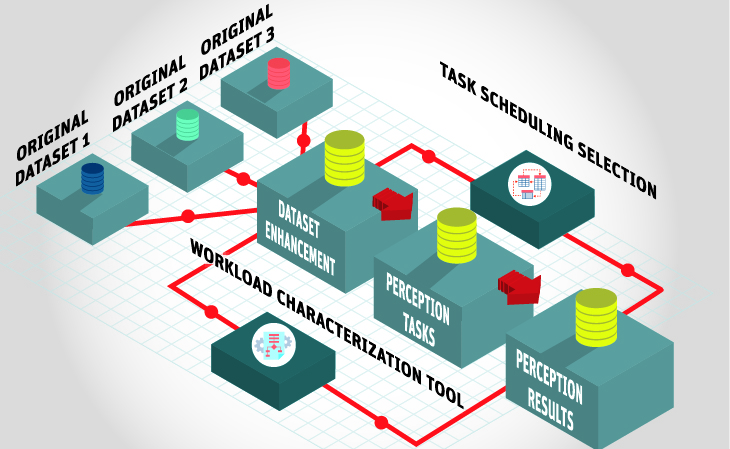
\includegraphics[width=\columnwidth, height=0.23\textheight]{CART-OnePiece2.jpg}
\caption{Integrated Approach}
\label{fig:proposed}
\end{figure}

In the context of autonomous driving, the characterization of the workload is essential to ensure that perception systems can operate within real-time constraints while maintaining reliability and safety. These systems perform a wide range of computation-intensive tasks, such as object detection, sensor fusion, and path planning, under strict latency thresholds \cite{Liu2023COLA:Systems}. In addition, efficient task scheduling is crucial due to the strict timing constraints and hard deadlines associated with autonomous driving tasks; missing a deadline can lead to severe accidents. 

%However, one of the most persistent challenges is defining appropriate performance indicators that allow a fair and consistent evaluation of ADV performance \cite{Kowalczyk2022EfficientVerification}. Without standardized metrics, comparing different solutions becomes ambiguous, undermining reproducibility and system optimization. Benchmarking efforts such as CAVBench \cite{wang2018} and \cite{Jambotkar2021AdaptiveImprovement} help address this by offering domain-specific evaluation criteria tailored to common workloads in ADV, but further refinement is needed to cover aspects such as scheduling policies and resource utilization.

A deeper understanding of system bottlenecks is also crucial, particularly in the early stages of the perception pipeline. Profiling studies show that real-time object detection algorithms often miss latency targets unless optimized for specific edge computing architectures \cite{Tang2022CharacterizationEdge}. Nonetheless, successful profiling continues to be challenging. This gap offers opportunities to optimize data preparation processes and improve overall system efficiency. As automotive systems move toward higher levels of autonomy and rely on increasingly heterogeneous data sources, the precise characterization of workload with powerful input datasets and task scheduling policy evaluation and benchmarking will be key to balancing accuracy, responsiveness, and computational resource use.

In this paper, we propose a novel integration approach to study the autonomous vehicle perception pipeline and task scheduling benchmarking called Cart-OnePiece present in Figure \ref{fig:proposed}. The generation and processing of synthetic datasets were integrated with the appropriate tools to analyze and characterize them. The datasets we can reproduce in the CARLA simulator \cite{dosovitskiy2017} from previous papers with the public code available on Github were chosen and enhanced by mimicking the Waymo perception dataset \cite{sun2020}. That choice first came because the CARLA simulator being the most popular and versatile open source ADV simulator and secondly because the dataset in \cite{sun2020} is the first large and multimodal real dataset collected with the Waymo prototype, a vehicle with millions of miles of test on the streets, which brings us close to the workload of real ADVs.

The new enhanced datasets were processed using the same tasks as its original dataset, resulting in perception results such as object detection or mapping. This processing is analyzed using workload characterization metrics. From this setup it was applied the StarPU \cite{Augonnet2011StarPU:Architectures}, a framework for task scheduling and workload characterization, that allowed for changing task scheduling predefined policies and even for the application of user task scheduling own policies creation allowing benchmarking it. For the best of our knowledge, the Cart-OnePiece is the first tool to integrate dataset generation, workload characterization and task scheduling analyses in one go to evaluate ADV perception computing systems. Thus, the main contribution of this paper is the integrated approach that provides datasets for ADV tasks for proper scheduling and characterization research works.

The remainder of this paper is organized as follows. Section 2 presents the background, Section 3 presents the methodology, Section 4 details the Experimental Setup, Section 5 shows the Experimental Analysis and Results, Section 6 discusses the related work, and finally, Section 7 describes our Conclusions and Future Work.

\section{Background}
This section provides an overview of the relevant concepts and software necessary to develop the proposed work.

\subsection{The Role of Datasets in Autonomous Vehicle Development}

The development of autonomous driving vehicles (ADV) is fundamentally based on robust perception systems capable of understanding highly dynamic and complex environments \cite{feng2020}. The effectiveness of these systems is directly proportional to the amount and quality of data used for their training and validation. Without extensive and high-quality datasets, the ability of ADVs to generalize across diverse scenarios remains severely limited.

%It is estimated that achieving a safety level comparable to human drivers would require driving billions of kilometers under varied conditions, a task that is practically impossible only through real-world tests \cite{angeletti2023}. This constraint has led to the widespread adoption of publicly available datasets and simulation-based synthetic data generation to accelerate development while maintaining safety and cost efficiency.

Early efforts like the Kitti dataset laid the foundation for ADV perception research by providing multimodal sensor data, including stereo cameras, LiDAR, and high-precision GPS/IMU. Kitti captured over 6 hours of diverse driving scenarios, covering urban, rural, and highway environments, and introduced benchmarks for stereo vision, optical flow, 3D object detection, SLAM, and visual odometry\cite{geiger2012,geiger2013} but has the drawback of being limited to one city only.

Recognizing the need for scale and diversity, Waymo Open Dataset (WOD) was introduced. WOD provides over 1150 scenes, each spanning 20 seconds, collected across different cities such as San Francisco, Phoenix, and Mountain View. It offers more than 12 million 3D LiDAR bounding box annotations and 9.9 million camera labels \cite{sun2020}. The WOMD-LiDAR dataset expands motion forecasting research by providing raw LiDAR data for more than 100,000 scenes, addressing limitations of previous datasets that only offered abstracted representations like bounding boxes \cite{chen2024}.  An extensive number of other open datasets in the real world prior to 2019 can be found in the survey by \cite{kang2019} and a more up-to-date review of available datasets can be found in \cite{liu2021} and \cite{liu2024}.

\begin{comment}
\begin{figure}[h]
\centering
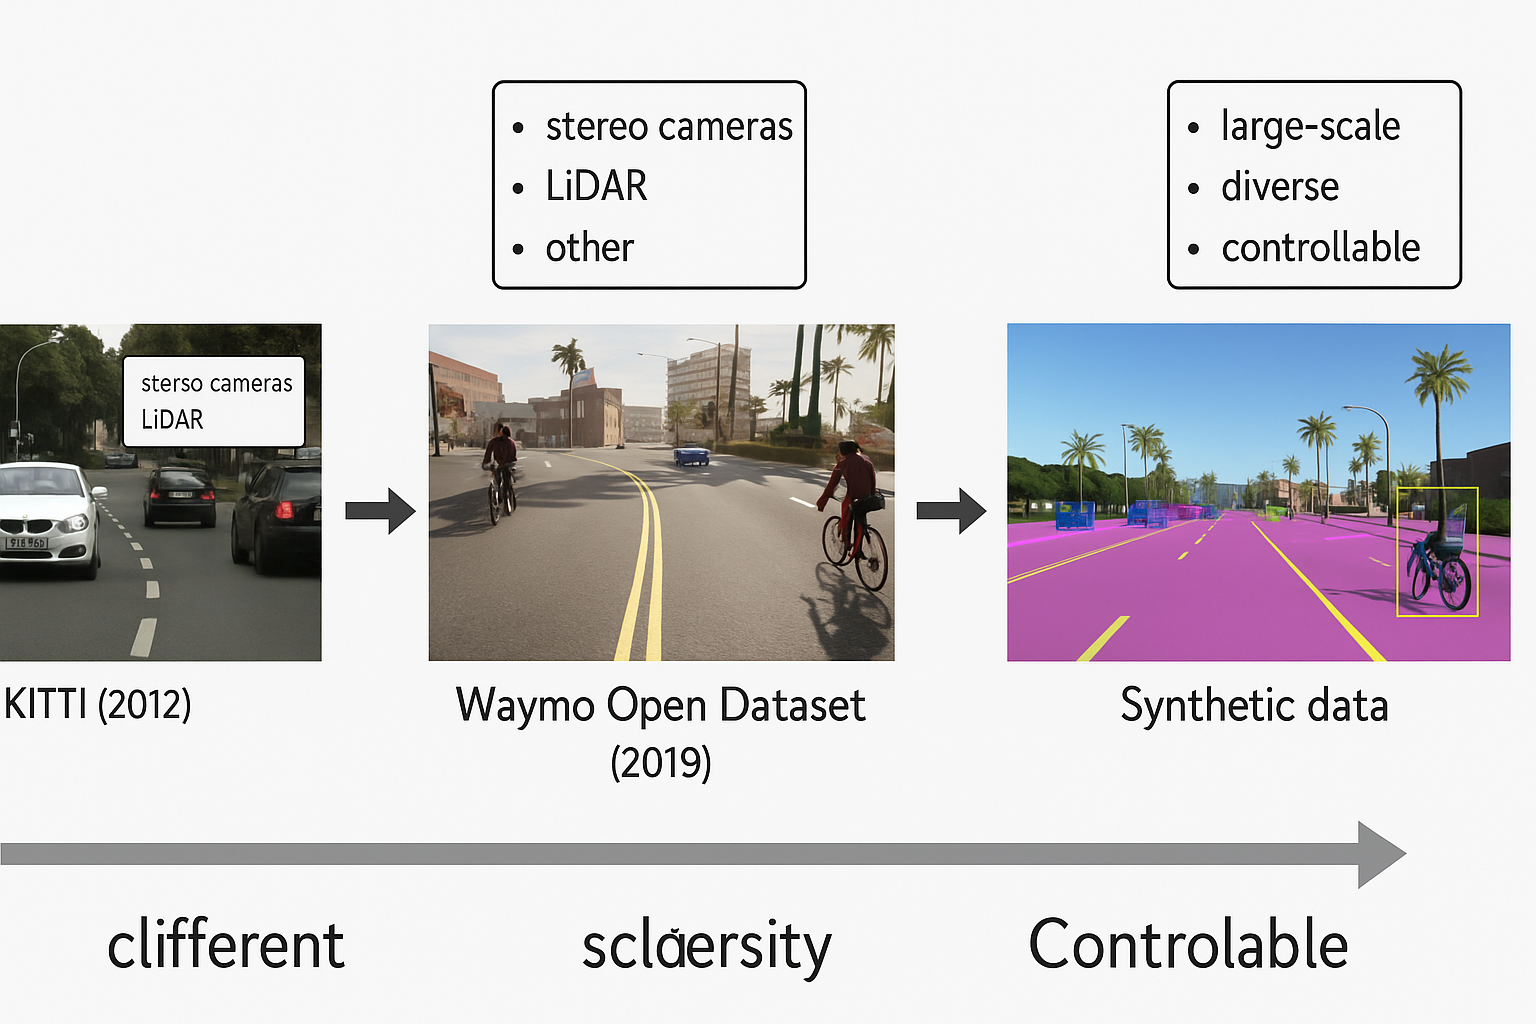
\includegraphics[width=\columnwidth]{fig2.png}
\caption{Real vs Synthetic Dataset}
\label{fig:your_label}
\end{figure}
\end{comment}

Real-world data collection can be expensive, time-consuming and challenging to scale \cite{feng2020}. Furthermore, real-world datasets often suffer from a long-tail distribution of scenarios, where rare but critical events such as accidents and unusual weather conditions are rarely presented \cite{song2024}. Gathering more data and corner cases is becoming more critical than inventing new deep neural network architectures. Collecting such data in the real world can be dangerous or infeasible. 

Therefore, synthetic datasets generated from 3D game engines, such as the CARLA simulator running on the Unreal Engine, offer a cost-effective and scalable alternative, allowing researchers to create customized scenarios and accelerate their research results. However, this introduces a new set of challenges: ensuring that synthetic data accurately reflect the complexities of the real world, including sensor noise, object textures, and physical dynamics.

\subsection{CARLA Simulator}

CARLA (Car Learning to Act) is an open-source urban driving simulator designed specifically for the research, development, and validation of autonomous driving systems. Unlike general-purpose simulators or gaming engines, CARLA was developed from the ground up to address the specific needs of the autonomous driving community, providing realistic urban environments, dynamic actors, and detailed sensor simulation \cite{dosovitskiy2017}. 


Its architecture is based on the Unreal Engine, allowing high-fidelity rendering, dynamic weather, and realistic physics. The open digital assets of CARLA include roads, buildings, vehicles, pedestrians and traffic elements, allowing researchers to simulate a wide range of real-world driving conditions with customizable sensor suites, such as RGB cameras, LiDAR, radar and semantic segmentation outputs \cite{deschaud2021}. Figure \ref{fig:CARLATown} shows a top view of the city used in this work.


\begin{figure}[h]
\centering
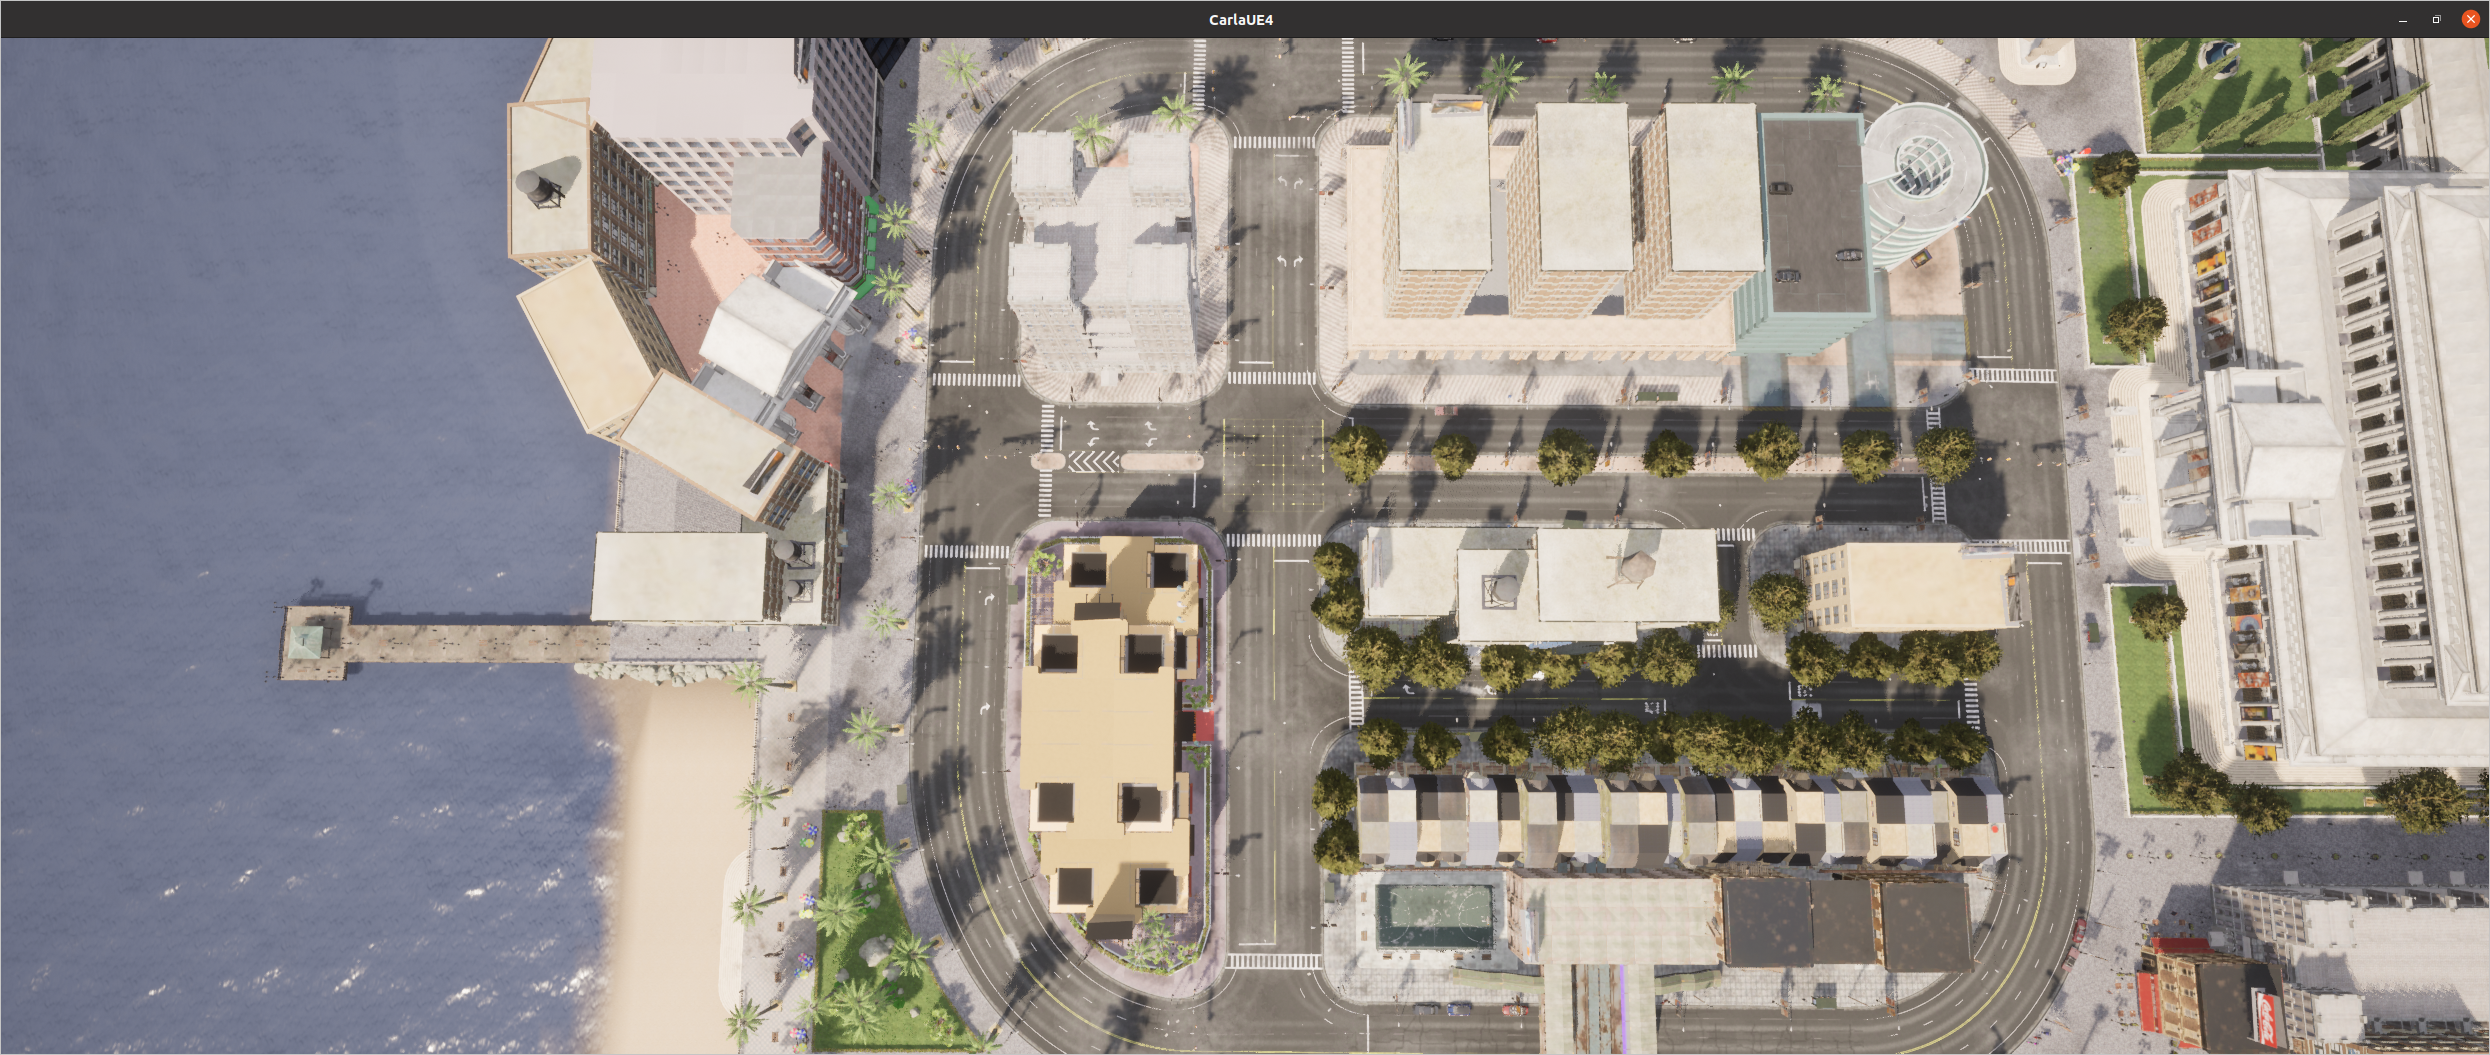
\includegraphics[width=\columnwidth]{fig4.png}
\caption{CARLA Town 10hd Top View}
\label{fig:CARLATown}
\end{figure}

The platform supports both classical modular driving pipelines and modern end-to-end learning approaches based on imitation learning or reinforcement learning. The flexibility to adjust environmental parameters, sensor configurations, and actor behavior has made CARLA a standard tool in academic and industrial ADV research \cite{gomez2022}.

Despite its advantages, CARLA does have some limitations. High computational demands, especially when running reinforcement learning frameworks or multi-actor simulations, can be a bottleneck. Issues such as lower simulation speeds compared to real time and the complexity of synchronizing large-scale distributed training architectures require sophisticated system engineering \cite{liu2023}. 


\subsection{ADV Perception System}


The perception system is a foundational component of an ADV, which allows it to understand and interpret its environment. Complete information on the hardware, software, and network systems of autonomous driving vehicles can be found in \cite{silva2024}. However, for the purposes of dataset creation, it is beneficial to focus specifically on the perception system itself represented in Figure \ref{fig:perceptionsystem}.

The perception system is responsible for processing raw sensor data to create a complete understanding of the vehicle's surroundings \cite{badue2021}. This involves several key steps, including data acquisition, sensor fusion, object detection, tracking, and scene understanding \cite{ahangar2021}. It relies on multimodal sensor configurations, typically combining cameras, LiDAR, radar, ultrasonic sensors, and GNSS/IMU. Cameras provide rich semantic information but are sensitive to lighting and weather. LiDAR offers precise 3D spatial mapping but struggles in fog, snow, or heavy rain. Radar complements these by being robust to adverse weather conditions, but has a lower resolution. Sensor fusion is therefore critical to compensate for individual sensor limitations \cite{yeong2021}. 

\
\begin{figure}[h]
\centering
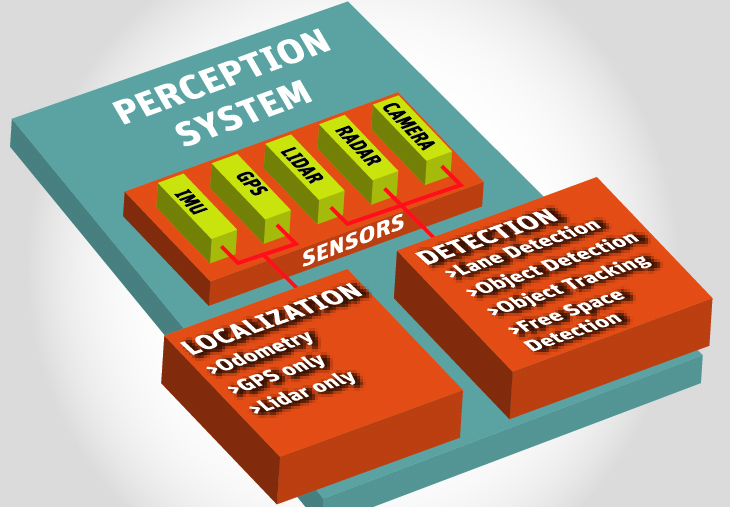
\includegraphics[width=\columnwidth, height=0.26\textheight]{Perception-System2.jpg}
\caption{ADV Perception System}
\label{fig:perceptionsystem}
\end{figure}

Data acquisition involves collecting raw sensor data from these various sensors. This data is then pre-processed to remove noise and correct for any sensor-specific distortions. The effectiveness of these systems is directly proportional to the amount and quality of data used for their training and validation, as without extensive and high-quality datasets, the ability of ADVs to generalize across diverse scenarios remains severely limited. This perception pipeline transforms data into information by imitating the human ability to perceive and formulate a reliable picture of the environment \cite{yeong2021}.

%Modern perception pipelines are generally composed of several stages that usually follow the sequence of sensor data acquisition, preprocessing and calibration, feature extraction, object detection, tracking, and scene understanding \cite{badue2021}. These stages feed into downstream modules such as localization, motion prediction, and planning. Recent studies show that perception performance still suffers under adverse environmental conditions. Visual-based perception, particularly camera-based systems, significantly degrades under fog, rain, or glare, leading to recognition errors and safety risks \cite{jiang2022}. This is a major challenge to achieve reliable Level 4 and 5 autonomy.


\subsection{ADV WorkLoad}

Autonomous vehicles are relying on complex computer systems to perceive their surroundings, plan their actions, and control the vehicle. The computational demands of these systems, often referred to as workload, are a critical factor in ensuring the safe and efficient operation of ADVs. Understanding and characterizing this workload is essential to optimize resource allocation, manage power consumption, and guarantee real-time performance. Accurately estimating the performance of perception systems requires models that consider available resources. 

These workloads are typically heterogeneous, involving a mix of tasks such as data acquisition, image preprocessing, neural network inference, and multisensor fusion, all of which must operate under strict real-time constraints. The performance of such systems is not solely dependent on algorithmic accuracy, but also on the ability to process data efficiently across different hardware architectures, including CPUs, GPUs, and specialized accelerators \cite{Tang2022CharacterizationEdge}.

The dynamic nature of driving environments introduces significant variability in workload. Factors such as traffic density, weather conditions, and the complexity of the surrounding environment can all impact the computational demands of ADV systems. 

%For example, driving in heavy traffic or adverse weather conditions requires more intensive processing of sensor data to accurately detect and track other vehicles and obstacles. Such variabilities may also contribute to burst computation and memory access, potentially leading to increased tail latency and impacting safety \cite{Liu2023COLA:Systems}

Characterizing the workload involves understanding the types of data being processed and the nature of the algorithms being used. As ADV applications are mainly focused on detection, recognition, and prediction, workloads often fall into the domains of computer vision, machine learning, and deep learning \cite{wang2018}. 

%Therefore, one of the main challenges in this domain lies in defining consistent performance indicators to compare algorithms in varying datasets and hardware setups \cite{Kowalczyk2022EfficientVerification}. Furthermore, recent studies highlight that preprocessing stages, such as image decoding, resizing, and sensor calibration, are often overlooked, despite contributing significantly to overall latency \cite{Bachkaniwala2024Lotus:Profiling}. 

%Effective workload management is essential to maintain the performance and safety of autonomous vehicles. This involves techniques such as dynamic task scheduling, resource allocation, and adaptive algorithm selection. By carefully characterizing and managing the workload, it is possible to optimize the performance of ADV systems, ensure timely responses to critical events, and ultimately achieve higher levels of driving automation.


\subsection{StarPU Framework for Task Scheduling and Workload Characterization}

%As autonomous driving systems integrate more complex perception and decision-making algorithms, efficient scheduling of computational workloads becomes critical. 

StarPU is a runtime system designed to simplify and optimize task scheduling and metrics measurement on heterogeneous computing platforms. It has a set of tools for online and offline performance metrics to characterize the tasks sent to the framework. It offers an API for implementing various scheduling algorithms. This framework works in conjunction with a distributed shared memory manager to optimize task mappings and data transfers, and to overlap communications with computations \cite{KasmiPerformanceArchitecture}.

StarPU provides a high-level, unified execution model coupled with a data management library. It allows developers to submit vehicle processing tasks as functions, simplifying the process of managing the computational workload \cite{Silva2025TaskRuntime}. StarPU can dynamically schedule tasks and manage their distribution across GPU and CPU processing nodes, using scheduling strategies available on the framework such as DMDA, HEFT, Work Stealing and Priority Based. In addition to built-in schedulers, StarPU provides an API that enables users to implement and plug in their own custom scheduling strategies. This is especially valuable in research contexts where novel scheduling heuristics or domain-specific constraints must be evaluated under real or simulated load conditions.

\begin{comment}
\begin{figure}[h]
\centering
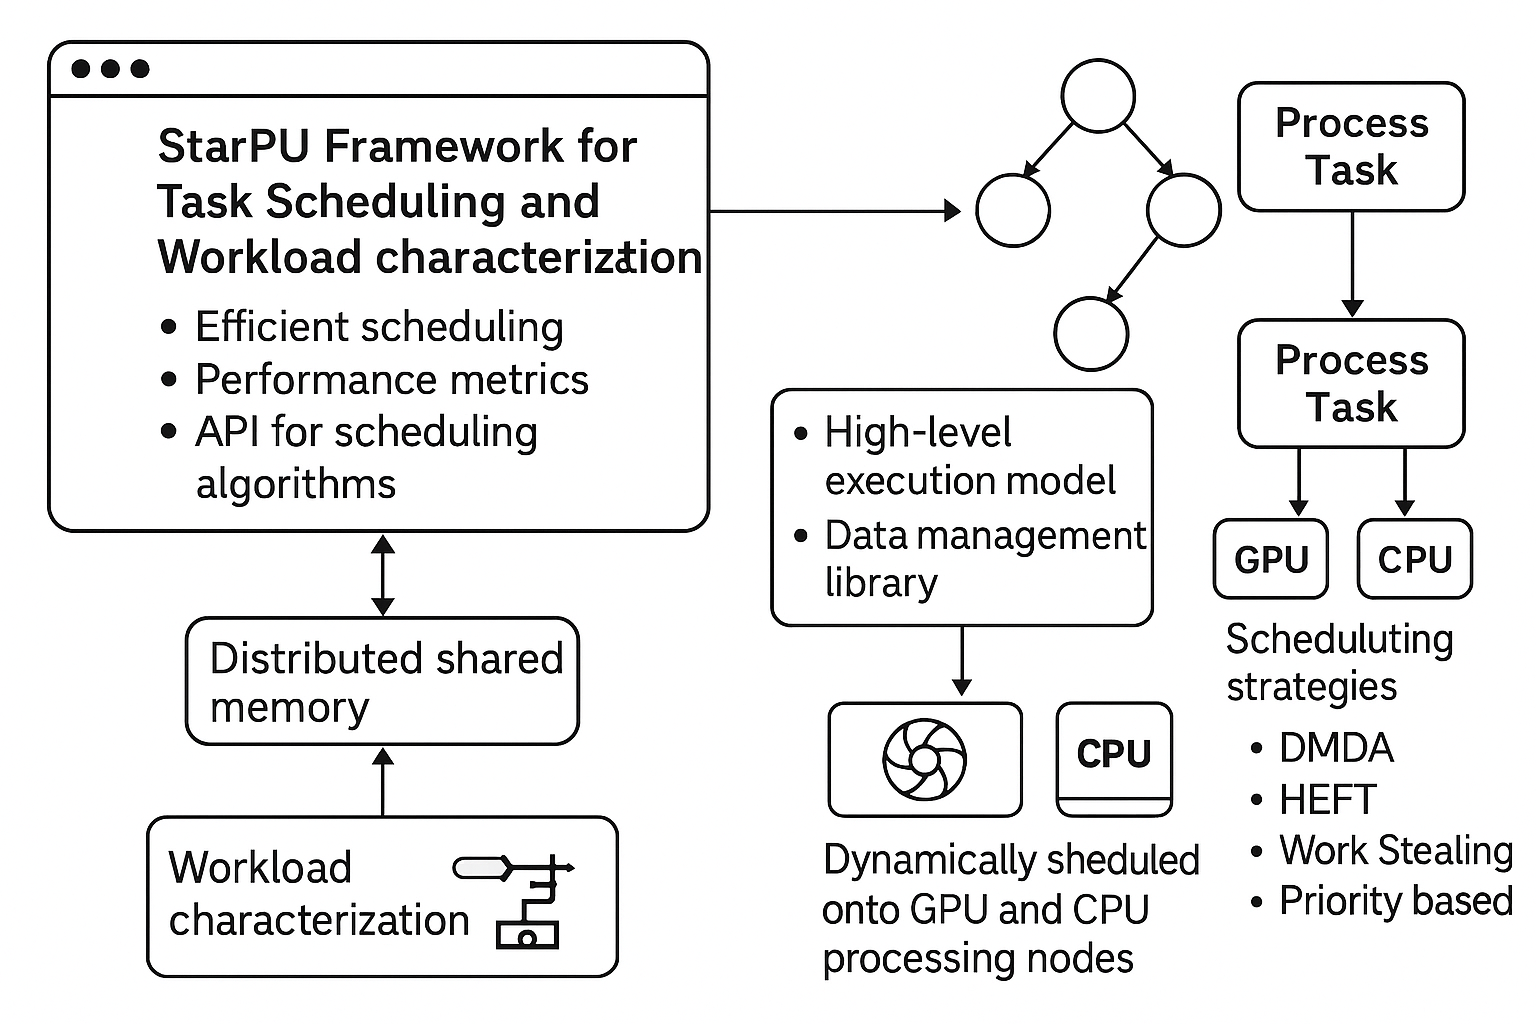
\includegraphics[width=\columnwidth]{fig5.png}
\caption{StarPU Framework}
\label{fig:your_label}
\end{figure}
\end{comment}

%In addition, the framework represents computational workflows as Directed Acyclic Graphs (DAGs), where nodes denote tasks and edges capture their dependencies. This structure allows the runtime to make informed scheduling decisions while balancing the load, optimizing the data locality, and minimizing memory transfers. The StarPU programming interface enables developers to define tasks with multiple implementations and declare data dependencies through access modes such as read, write, and read-write \cite{Miletto2019}. These mechanisms ensure that tasks are executed in an order that respects both computational and memory constraints.

Moreover, it facilitates workload characterization through its support for runtime tracing and performance monitoring. By instrumenting execution traces, it enables the collection of granular metrics on task start times, durations, device assignments, and memory usage. These logs are visualized via tools like StarVZ and Paje Tracer, which offer intuitive performance dashboards to identify bottlenecks, analyze task queue latency, and observe task distribution across devices.

\section{Methodology}

This section details the integrated methodology developed to enable the enhancement of the dataset, the characterization of perception workload, and the benchmarking of task scheduling in autonomous driving vehicles. 

\subsection{Dataset Enhancement}

As the objective is to have a close to real dataset generated in a working ADV prototype that would give enough workload to be relevant to analyze, it was chosen to mimic the setup of the Waymo ADV \cite{waymo_website}. The choice comes from the fact that it is one of the most advanced working prototypes in the world giving rides in many cities in the United States. It also has a public dataset generated by a real sensor suit available and described in \cite{sun2020}. Furthermore, we were looking for datasets generated in the CARLA simulator due to the benefits mentioned in the previous section and, that the script is available on Github. Starting the search from the ADV dataset review papers\cite{liu2024,song2024,liu2021} it was initially chosen a set of papers \cite{Deschaud2021Kitti-CARLA:Simulator,deschaud2021,DeLaPena2022ADROS,Jang2022Carfree:Simulator,Nesti2024CARLA-GeAR:Models, Han2023CARLA-Loc:Environments,Wielgosz2023CARLA-BSP:Pedestrians} that the sensor setup can be seen in Table \ref{tab:dataset_sensors}. 

After analyzing these papers, the AD PerDevKit and the CARLA-Loc papers use CARLA only to display the simulation, but all the data are generated in the Robot Operating System (ROS) that is linked to CARLA so these were discarded. In addition, the CARLA-BSP is specific for detecting pedestrians, so it was not used as well. Paris CARLA main focus is on LiDAR data processing and is from the same author from Kitti-CARLA so it was also not used.  Hence, the Kitti-CARLA, Carfree and CARLA-GeAR were the selected papers with datasets that would be reproduced and enhanced in this work. 

\begin{table}[ht]
  \centering
  \caption{Sensors per Dataset (Real Waymo vs Synthetic Datasets)}
  \label{tab:dataset_sensors}
  \renewcommand{\arraystretch}{1.9}
  \setlength{\tabcolsep}{0.1pt}

  % fonte +1 pt (10 → 11) e tabela adaptável
  {\fontsize{7pt}{6pt}\selectfont
  \begin{tabularx}{\columnwidth}{@{}P{2.0cm}*{3}{P{2.2cm}}@{}}
    \toprule
    \rowcolor{myblue}
    \textbf{Dataset} & \textbf{Cameras} & \textbf{LiDAR} & \textbf{Radar} \\
    \midrule
    Waymo Open      & 5 RGB (360°)            & 5 scanners (roof + 4 SR) & — \\
    Kitti–CARLA     & 2 RGB                   & 1 HDL-64E               & — \\
    Paris–CARLA–3D  & Ladybug5 (6 RGB)        & 1 HDL-32E               & 1 FMCW \\
    AD PerDevKit    & 6 RGB ring + extras     & 1 64-beam               & — \\
    CarFree         & 1 RGB front             & 1 RGB                   & — \\
    CARLA–BSP       & 1 RGB + semantic        & Stereo RGB              & 3 Falcon 773 \\
    CARLA–GeAR      & Stereo RGB              & 1 HDL-32E               & 3 Falcon 773 \\
    \bottomrule
  \end{tabularx}}
\end{table}




\begin{table*}[!htbp]              % ➊ use table* se realmente precisar de duas colunas
\centering                        % ➋ centraliza a caixa da tabular
\footnotesize
\caption{Perception Tasks in Selected Datasets}
\label{tab:DatasetPerception}
\renewcommand{\arraystretch}{1.5} % altura das linhas
\setlength{\tabcolsep}{4pt}       % espaçamento horizontal
\rowcolors{2}{white}{gray!10}

% ➌ se não precisar de quebra automática, troque tabularx por tabular
\begin{tabular}{>{\columncolor{myblue}}l|c|c|c|c|c|c}
  \rowcolor{myblue}
  \textbf{Dataset} & \textbf{2D Det.} & \textbf{3D Det.} &
  \textbf{Sem. Segm.} & \textbf{Inst. Segm.} &
  \textbf{Tracking} & \textbf{Adv. Eval.} \\
  Waymo       & F‑RCNN   & P.Pillars  & --      & --       & --        & --         \\
  Kitti‑CARLA & PSPNet   & --         & PSPNet  & --       & LOAM/OS2  & --         \\
  CarFree     & YOLOv3   & --         & --      & --       & DeepSORT  & --         \\
  CARLA‑GeAR  & YOLOv3   & StereoRCNN & DLabv3+ & DeepSORT & --        & Patch Gen. \\
\end{tabular}
\end{table*}



\begin{table}[ht]
  \centering
  \caption{Main Perception Tasks in Selected Datasets}
  \label{tab:DatasetTasksPerception}
  % --- mesmo tamanho de fonte da Tabela 2 ---
  \footnotesize
  % --- mesma altura de linha da Tabela 2 ---
  \renewcommand{\arraystretch}{1.5}
  \setlength{\tabcolsep}{4pt}

  \rowcolors{2}{white}{gray!10}
  \begin{tabularx}{\columnwidth}{@{}>{\columncolor{myblue}}l|X@{}}
    \toprule
    \rowcolor{myblue}
    \textbf{Dataset} & \textbf{Main Tasks} \\ \midrule

    \multirow[t]{2}{*}{Waymo} &
      2D/3D Detection \\*[-3pt] % pequeno recuo para colar linhas
      & Vehicle Tracking \\ \addlinespace

    \multirow[t]{2}{*}{Kitti--CARLA} &
      Semantic/instance segmentation \\*[-3pt]
      & LiDAR/image odometry \\ \addlinespace

    CarFree & 2D Vehicle/Pedestrian detection \\ \addlinespace

    \multirow[t]{2}{*}{CARLA--GeAR} &
      Pedestrian detection \\*[-3pt]
      & 2D/3D vehicle pose estimation \\

    \bottomrule
  \end{tabularx}
\end{table}




Although the Waymo ADV is composed of around 29 sensors from LiDARs, Radars, and Cameras, the Waymo Perception Dataset uses only five cameras and one Lidar, all mounted in the top of the vehicle. Thus, the selected datasets were equalized with this number of LiDAR and cameras which are distributed facing left, front-left, front, front-right, and right. The necessary code update and adaptations were made in each of the selected datasets. 

%A sample of the collected data can be seen in Figure \ref{fig:Sensor Caption}

\begin{comment}
\begin{figure}[h]
\centering
\fbox{\rule{0pt}{2in} \rule{0.9\columnwidth}{0pt}} % 2in height, column width
\caption{Sensors Caption Example (Placeholder)}
\label{fig:Sensor Caption}
\end{figure}
\end{comment}

\subsection{Applied Perception Tasks}


In Table \ref{tab:DatasetPerception} a table of the main perception tasks performed in each dataset is presented. In addition, Table \ref{tab:DatasetTasksPerception} shows detailed information with the algorithms applied to each task performed by the perception systems in each dataset against the Waymo dataset.

Furthermore, not every task is performed on every paper. It was decided to keep the selected datasets performing the same tasks that they performed originally but doing that for each sensor, increasing the number of workload necessary multiplied by the number of sensors increased in the dataset enhancement phase of this work. In the next paragraphs, it will be described in more detail the tasks applied in the perception system of each selected dataset.

The Kitti-CARLA dataset \cite{Deschaud2021Kitti-CARLA:Simulator} replicates the Kitti dataset within the CARLA simulator, aiming to provide high-fidelity synthetic data that reflect real-world conditions. It supports tasks such as monocular depth estimation, object detection, and semantic segmentation. The dataset is specifically designed for benchmarking perception algorithms that rely on camera-based and LiDAR modalities. The authors implemented pipelines based on deep learning architectures, such as YOLO for object detection and UNet for segmentation.

Carfree \cite{Jang2022Carfree:Simulator} uses CARLA’s simulation capabilities to automatically label scenes, drastically reducing the need for human annotation. Carfree supports object detection tasks and applies RetinaNet and Faster R-CNN as baseline detection models to validate the utility of the dataset. This setup allows researchers to explore detector performance across diverse scenes, emphasizing efficiency in training and evaluation without compromising detection accuracy.

The CARLA-GeAR \cite{Nesti2024CARLA-GeAR:Models} dataset is designed to evaluate adversarial robustness in visual perception tasks. Provides adversarial and clean image pairs to benchmark model robustness under challenging conditions. This dataset supports classification and object detection tasks, using models such as ResNet-50 and YOLOv3 to evaluate performance degradation under adversarial perturbations. It is particularly useful for testing the security and stability of vision-based perception systems in autonomous vehicles.

\subsection{ADV Workload Characterization}

%Workload characterization is essential for optimizing the performance and safety of autonomous vehicles. By understanding the specific demands that perception tasks place on the underlying hardware, we can design scheduling strategies and resource allocation policies to maximize efficiency. ADV perception pipelines exhibit a distinctive execution profile: they process a continuous stream of high‑bandwidth sensor data and must transform it into a consistent world model within a hard real‑time budget.  Because a single missed deadline can translate into unsafe behavior, recent characterization studies have converged on evaluation with a focus on latency, complementing it with resource utilization and information on energy consumption to better explain and eventually predict timing failures. 

To effectively characterize the ADV workload, it is crucial to identify key metrics that capture the demands of the perception system resources. Common metrics include CPU utilization, memory footprint, memory bandwidth, and I/O bandwidth \cite{wang2018}. Furthermore, the latency of individual modules within the perception pipeline, such as object detection and semantic segmentation, provides valuable information about their computational complexity \cite{Liu2023COLA:Systems, Gog2021Pylot:Vehicles}. Memory access patterns can also be insightful, as some applications have phases of memory access, causing a surge in memory bandwidth requirement followed by a computation phase \cite{Tang2022CharacterizationEdge}. Table \ref{tab:adv-char-summary} summarizes the papers used to define the metrics to be used in this work.

\begin{table*}[!htbp]
  \centering
  \caption{Summary of ADV Workload Characterization Studies}
  \label{tab:adv-char-summary}
  \renewcommand{\arraystretch}{1.5}
  \setlength{\tabcolsep}{4pt}
  \resizebox{\textwidth}{!}{%
  \rowcolors{2}{white}{gray!10}       % zebra striping for body rows
  \begin{tabular}{@{}p{0.4\linewidth} p{.25\linewidth} p{.25\linewidth}@{}}
    \toprule
    \rowcolor{myblue}
    \textbf{Paper} & \textbf{Workload Components} & \textbf{Metrics} \\
    \midrule
    % ──────────────────────────────────────────────────────────────────
    COLA: Characterizing and Optimizing the Tail Latency for Safe Level-4 Autonomous Vehicle Systems\,\cite{Liu2023COLA:Systems} &
    End-to-end Level-4 AV pipeline (perception, planning) &
    Tail / average latency; safety (crash rate) \\[0.5em]
    % ──────────────────────────────────────────────────────────────────
    Adaptive Optimization of Autonomous-Vehicle Computational Resources for Performance and Energy Improvement\,\cite{Jambotkar2021AdaptiveImprovement} &
    Multi-subsystem (perception, control, planning) &
    Detection latency; accuracy (precision); energy \\[0.5em]
    % ──────────────────────────────────────────────────────────────────
    Efficient Characterization Method for Big Automotive Datasets Used for Perception System Development and Verification\,\cite{Kowalczyk2022EfficientVerification} &
    Dataset scene elements (static + dynamic objects, trajectories) &
    Scene complexity (object density; trajectory metrics); distribution distance (Wasserstein) \\[0.5em]
    % ──────────────────────────────────────────────────────────────────
    CAVBench: A Benchmark Suite for Connected and Autonomous Vehicles\,\cite{wang2018} &
    Six AV apps: SLAM, object detection (2D/3D), tracking, battery monitoring, speech, video analysis &
    Execution-time breakdown; QoS vs. resource curves; memory bandwidth; cache miss rates \\[0.5em]
    % ──────────────────────────────────────────────────────────────────
    Characterization of Real-Time Object Detection Workloads on Vehicular Edge\,\cite{Tang2022CharacterizationEdge} &
    Single-module object-detection workloads on vehicular edge &
    Inference latency (FPS); GPU/CPU utilization; memory usage; accuracy \\[0.5em]
    % ──────────────────────────────────────────────────────────────────
    Chauffeur: Benchmark Suite for Design and End-to-End Analysis of Self-Driving Vehicles on Embedded Systems\,\cite{Maity2021Chauffeur:Systems} &
    Embedded AV-pipeline tasks (detection, SLAM, control) &
    Latency; throughput; resource usage (CPU/GPU) \\[0.5em]
    % ──────────────────────────────────────────────────────────────────
    Pylot: A Modular Platform for Exploring Latency–Accuracy Trade-offs in Autonomous Vehicles\,\cite{Gog2021Pylot:Vehicles} &
    Modular AV pipeline in CARLA (perception, planning) &
    Module latency vs. accuracy (AP); end-to-end safety impact \\[0.5em]
    % ──────────────────────────────────────────────────────────────────
    Edge AIBench 2.0: Benchmarking Intelligent Edge Scenarios for Connected and Autonomous Vehicles\,\cite{Hao2022EdgeSystems} &
    Critical AV tasks (e.g., lane-keeping, perception) across IoT–Edge–Cloud tiers &
    Throughput; 99th-percentile latency \\
    % ──────────────────────────────────────────────────────────────────
    \bottomrule
  \end{tabular}
  }
\end{table*}



%A recurring issue highlighted in recent studies is the impact of tail latency and resource contention on the performance of autonomous vehicle workloads. However, most existing approaches fail to offer a unified tool chain capable of linking different performance dimensions, such as task queue delays, processor utilization, cache behavior, and energy consumption, in a coherent way. This gap is addressed by StarPU, which provides built-in support for online performance counters, fine-grained execution traces (FxT) and optional integration with the performance API for low-level hardware events. These capabilities allow StarPU to trace the entire chain of performance effects, from scheduler decisions down to microarchitectural outcomes. Our methodology takes advantage of these built-in probes to profile the perception pipeline.

%In this work, it is applied both on-line and off-line metrics to profile the perception system workload. Table \ref{tab:StarPU_metrics} summarizes the metric families that were recorded for every scheduler under test and shows how it is extracted from StarPU.  We deliberately restrict the set to metrics that are both schedulable meaning that affected by the ordering of tasks and actionable that are the ones directly usable when deciding whether a new policy is better.

\begin{comment}
\begin{table*}[h]
  \centering
  \caption{Metric suite and StarPU‐based acquisition workflow}
  \label{tab:StarPU_metrics}
  \begin{tabular}{@{}p{1.3cm}p{3.2cm}p{6.5cm}p{4.5cm}@{}}
    \toprule
    \textbf{Family} & \textbf{Metric} & \textbf{Extraction path} & \textbf{Rationale} \\
    \midrule
    \textbf{Timing}
      & Mean and P95/P99 latency for every frame; end‐to‐end jitter; deadline‐miss count 
      & Task timestamps \(\rightarrow\) FxT → percentile calculator 
      & Direct indicator of safety margin~\cite{Liu2023COLA:Systems} \\
    \addlinespace
    \textbf{Throughput}
      & Frames · s\(^{-1}\) (effective tasks · s\(^{-1}\))
      & Worker counter \texttt{w\_total\_executed} / elapsed time 
      & Caps camera rate or UI/MMW spin rate \\
    \addlinespace
    \textbf{Utilization}
      & CPU thread utilization; CPU SM occupancy; ready queue depth
      & \texttt{StarPU\_WORKER\_STATS} trace viewer
      & Detects load imbalance and hidden stalls \\
    \addlinespace
    \textbf{Memory \& I/O}
      & Aggregate memory bandwidth (GB · s\(^{-1}\)); bus transfers; cache/TLB MR
      & \texttt{StarPU\_BUS\_STATS}, PAPI counters 
      & Explains latency spikes due to contention~\cite{wang2018} \\
    \addlinespace
    \textbf{Energy}
      & Joules per frame; mean board power (W)
      & \texttt{StarPU\_ENERGY\_PROFILE} with PAPI, INA231 
      & Quantifies latency–energy trade‐off~\cite{Jambotkar2021AdaptiveImprovement} \\
    \addlinespace
    \textbf{Accuracy guard}
      & mAP / IoU of detection output
      & Offline COCO evaluation scripts; site‐specific
      & Ensures timing slack does not degrade perception quality \\
    \bottomrule
  \end{tabular}
\end{table*}
\end{comment}

In practice, every workload variant was run with the following environment flags presented in Table \ref{tab:StarPU-flags}. During execution, StarPU prints a concise end‑of‑run report listing, for each worker, the fraction of time spent executing, waiting, or scheduling, together with its achieved GFLOP.  These numbers feed directly into the utilization and throughput metrics.  The FxT file is then converted with the \texttt{StarPU\_fxt\_tool} and visualized in ViTE. Table \ref{tab:StarPU-files} shows the generated files and the information contained in each of them.

\begin{table}[ht]
  \centering
  \caption{Key StarPU Environment Flags and Effects}
  \label{tab:StarPU-flags}
  \renewcommand{\arraystretch}{1.5}
  \resizebox{\columnwidth}{!}{%
  \rowcolors{2}{white}{gray!10} % Zebra striping from second row (white, light gray)
  \begin{tabular}{@{}p{0.4\linewidth} p{0.55\linewidth}@{}}
    \toprule
    \rowcolor{myblue}
    \textbf{{Environment Flag}} & \textbf{Purpose} \\
    \midrule
    \texttt{StarPU\_PROFILING=1}       & per-task start/end timestamps \\
    \texttt{StarPU\_FXT\_TRACE=1}      & event trace for ViTE (Paje) \\
    \texttt{StarPU\_WORKER\_STATS=1}   & on-line worker utilisation summary \\
    \texttt{StarPU\_BUS\_STATS=1}      & memory-traffic counters \\
    \bottomrule
  \end{tabular}
  }
\end{table}


\begin{table}[ht]
  \centering
  \caption{StarPU Output Trace Files and Main Contents}
  \label{tab:StarPU-files}
  \renewcommand{\arraystretch}{1.5}
  \rowcolors{2}{white}{gray!10} % Zebra striping from second row (white, light gray)
  \begin{tabular}{@{}p{0.34\linewidth} p{0.63\linewidth}@{}}
    \toprule
    \rowcolor{myblue}
    \textbf{File} & \textbf{Contents and Purpose} \\
    \midrule
    \texttt{tasks.rec}         & Record of every task executed, including JobId, submission order, assigned WorkerId, and timestamps for submission, start, and completion. \\
    \texttt{sched\_tasks.rec}  & Trace of scheduling events (e.g., when tasks are pushed to or popped from the ready queue). \\
    \texttt{activity.data}     & Timeline of worker activity (idle or executing) over time for each worker. \\
    \texttt{distrib.data}      & Per-task execution duration summary; typically lists each task’s runtime. \\
    \texttt{trace.rec}         & Detailed event trace including state transitions, used for fine-grained timeline visualization or debugging. \\
    \bottomrule
  \end{tabular}
\end{table}


Integration with the CARLA simulator allows controlled experimentation and the generation of synthetic data that closely mimic real-world driving scenarios. By varying environmental conditions, traffic patterns, and sensor configurations, we can create diverse workload scenarios and assess the performance of the perception system under different operating conditions. This approach enables us to identify performance bottlenecks and evaluate the effectiveness of different scheduling strategies.

Data collected through online monitoring and offline tracking will be analyzed using statistical techniques to identify key trends and patterns in workload \cite{King1986WORKLOADCHARACTERIZATION}. Descriptive statistics, such as mean, variance, and percentiles, will be used to summarize the use of resources of different perception tasks. Furthermore, visualization techniques will be employed to identify correlations between workload characteristics and system performance \cite{https://doi.org/10.1002/cpe.4472}. This analysis will provide valuable information on the computational demands of the perception system and inform the development of optimized resource allocation and scheduling strategies within StarPU.


\subsection{Task Scheduling Benchmarking}

To accurately evaluate the performance and efficacy of different task scheduling strategies in the ADV perception pipeline, a structured benchmarking approach was devised utilizing the StarPU runtime system. StarPU was selected for its ability to handle diverse scheduling policies, ease of integration with heterogeneous hardware resources (CPUs and GPUs) and comprehensive support for on-line and off-line workload characterization metrics.

The necessary choice to use Python language to seamlessly integrate StarPU to CARLA limited the choices of online characterization APIs available in StarPU that are much more vast when programming in C or C++ in it, but still some functions to collect online data. It did not affect the offline performance analyzes of the script execution, which basically uses traces of the online execution.

Three different dataset generation pipelines mentioned previously, CarFree, KittiCARLA, and CARLA-GeAR, were systematically evaluated. Each pipeline utilizes the CARLA simulator to generate synthetic perception data, but differs in terms of data characteristics and processing tasks:

\begin{itemize}
\item \textbf{CarFree}: Focuses on bounding box extraction and pedestrian detection tasks.
\item \textbf{Kitti-CARLA}: Emphasizes point cloud generation and georeferencing, mimicking the Kitti dataset.
\item \textbf{CARLA-GeAR}: Integrates complex environmental interactions and detailed sensor simulations, emphasizing the generation of diverse scenarios.
\end{itemize}

Benchmarking scripts specific to each pipeline were developed to automate and standardize evaluations across multiple StarPU scheduling strategies, including eager, dequel mode (dm), dm with data awareness (dmda), work-stealing (ws), random, local ws (lws), priority-based (prio) and heterogeneous prio (heteroprio) schedulers. Each scheduler was evaluated under identical conditions defined by parameters such as capture loop iteration (set at 10 iterations), maximum frames (set at 3000 frames), and operational mode (both data extraction and generation mode) to ensure consistency across test runs.

Profiling was meticulously performed using environment flags provided by StarPU, such as 
\texttt{StarPU\_PROFILING}, \texttt{StarPU\_WORKER\_STATS}, and \texttt{StarPU\_FXT\_TRACE}. These profiling tools facilitated comprehensive data collection on metrics such as task execution times and worker efficiency. Results from each scheduler run were systematically aggregated into structured CSV files, followed by dedicated scripts for visualization and comparative analysis. These metrics were analyzed between the three datasets generation scripts enabling detailed observations into the behavior of different schedulers under varying data processing workloads.

Additional detailed profiling via FxT (Fine-Grained Execution Trace) logs, worker statistics, and task dependency visualizations enhanced the interpretability of the performance results. This comprehensive methodology allows for clear identification of bottlenecks, resource utilization patterns, and performance characteristics unique to each dataset pipeline.

%Ultimately, this benchmarking methodology ensures a comprehensive and reproducible framework, allowing precise comparative analysis of task scheduling strategies to identify optimal configurations optimized for real-time ADV perception system performance.


\section{Experimental Setup}
This section details the experimental infrastructure and configurations used to evaluate workload profiling and task scheduling performance using the Cart-OnePiece.

\subsection{System Hardware and Software}
The experimental evaluation was conducted using two distinct computational setups to comprehensively assess performance across varying hardware configurations.

The first machine setup consists of a compact workstation equipped with an Intel Core i5-10400 CPU featuring 6 cores and 12 threads, complemented by 64 GB of RAM. It is equipped with an NVIDIA GeForce RTX 3060 GPU with 12 GB of dedicated memory. The second machine setup consists of a high-performance system featuring an Intel® Core™ i9-14900K CPU with 24 cores (8 performance cores and 16 efficiency cores), supporting up to 32 threads, and paired with 64 GB of RAM. It integrates a NVIDIA Geforce RTX 4090 GPU with 24 GB of dedicated memory. %and provides extensive storage through two 2 Gb NVMe SSDs. Figure \ref{fig:setup1} and fig\ref{fig:setup2} shows the two machine configurations in detail.

\begin{comment}
    
\begin{figure*}[htbp]
  \centering
  \begin{minipage}[b]{0.45\textwidth}
    \centering
    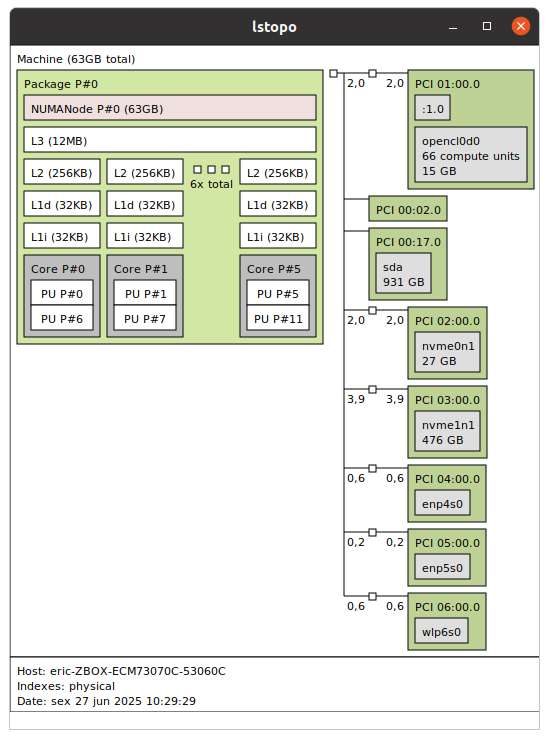
\includegraphics[width=\linewidth,height=7cm]{ZotacZbox.png}
    \caption{Computational Setup 1}
    \label{fig:setup1}
  \end{minipage}
  \hfill
  \begin{minipage}[b]{0.45\textwidth}
    \centering
    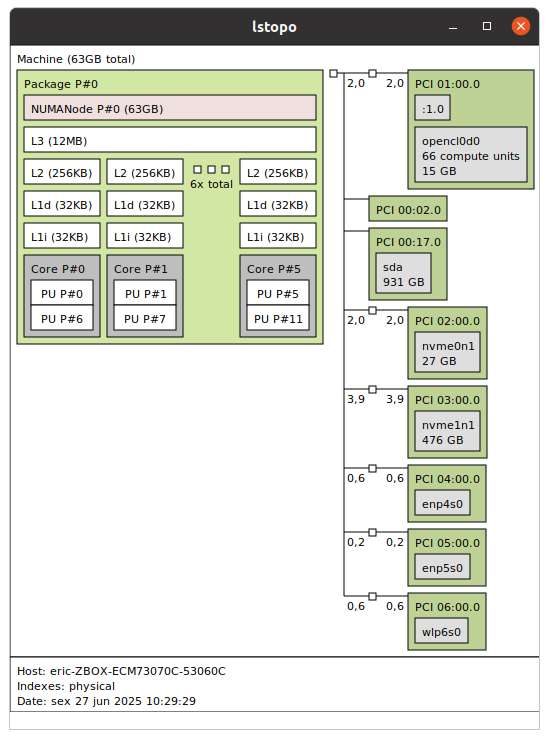
\includegraphics[width=\linewidth,height=7cm]{ZotacZbox.png}
    \caption{Computational Setup 2}
    \label{fig:setup2}
  \end{minipage}
\end{figure*}

\end{comment}

Both systems were configured with Ubuntu 20.04 as the operating system and utilized the CARLA simulator version 0.9.15 to simulate the ADV and collect data for the Datasets. Task scheduling and profiling were performed using StarPU version 1.4.99.%, which supports extensive profiling and task scheduling across heterogeneous computing resources (CPU and GPU).


\subsection{StarPU Setup}
\label{AA}

The developed application integrates the CARLA simulation environment with the StarPU runtime to efficiently handle task scheduling and workload profiling. The workflow across all dataset generation scenarios is structured to clearly distinguish between simulation management and setup tasks, executed independently of StarPU, and real world ADV tasks that are offloaded to StarPU for optimized execution.

In the CarFree scenario, StarPU handles the computational tasks involving the extraction and writing of pedestrian and vehicle bounding boxes. Specifically, bounding box coordinates extracted from simulation frames are encapsulated into dedicated StarPU tasks, where file-writing operations are managed asynchronously also with StarPU to optimize parallelism and resource utilization.

The Kitti-CARLA scenario utilizes StarPU primarily to parallelize computationally demanding georeferencing tasks associated with point cloud data. Each PLY file containing raw point cloud data generated from simulated LiDAR sensors is processed as a distinct StarPU task. These tasks transform raw sensor data into accurately georeferenced point clouds, handling large-scale computations efficiently.

For the CARLA-GeAR pipeline, StarPU's responsibilities include complex bounding box calculations and sensor data integration. The tasks managed by StarPU involve detailed processing of depth maps, bounding box projections, and occlusion calculations from multiple sensor modalities. This enables efficient processing of high-resolution simulation data, necessary for creating realistic perception scenarios.

In all scenarios, simulation initialization, actor management (vehicle, pedestrians), sensor setup, and world synchronization occur outside of the scope of StarPU. The role of StarPU is explicitly limited to tasks that would occur in the real ADV prototype, using its capabilities for scheduling, task distribution, and detailed profiling in that portion of the script. %This clear separation ensures that StarPU is profiling data similar to what is processed in a real driving scenario.



\section{Experimental Analysis and Results}

Some of the Cart-OnePiece features are presented in this section. Although much more data and insights could be provided, some basic usage was chosen and briefly analyzed to show the validation of our proposed tool.


\subsection{Cart-OnePiece as a Machine Evaluation Tool}

The simulations are run on both machines with the same script and collection setup for each dataset generator. The main findings are summarized in Table \ref{tab:perf_metrics} detailing the total number of tasks (\#Tasks), total execution time ($T_{\textsubscript{tot}}$~[s]), average task execution time ($Task_{\textsubscript{avg}}$~[s]), average wait time in the task queue ($Wait_{\textsubscript{avg}}$~[s]), and CPU utilization providing insights into how each perception workload behaves under different hardware capabilities.

It is important to point out that the CPU utilization is a fraction of the total, as the machines are running the OS and many simulation tasks from CARLA are not parsed to StarPU as explained before. But still showing important information about what could be gained with a more powerful high performance machine. StarPU measurement tools in Python do not separate the system processing measurements, but do profile in detail the tasks submitted into it. In addition, for these analyzes, we kept the same scheduling policy in all experiments, which was LWS. This strategy is very naive and evenly distributes workload between all processing units.


\begin{table}[ht]
  \centering
  \caption{Performance Metrics by Script and Machine}
  \label{tab:perf_metrics}
  \renewcommand{\arraystretch}{1.5}
  \setlength{\tabcolsep}{5pt}
  \resizebox{\columnwidth}{!}{%
  \rowcolors{2}{white}{gray!10}
  \begin{tabular}{@{}l l *{5}{P{1.3cm}} @{}}
    \toprule
    \rowcolor{myblue}
    \textbf{Script} & \textbf{HW} & \textbf{\#Tasks} & \textbf{T\textsubscript{tot} [s]} & \textbf{Task\textsubscript{avg} [s]} & \textbf{Wait\textsubscript{avg} [s]} & \textbf{CPU util.} \\
    \midrule
    \multirow[t]{2}{*}{Carfree}    & I5 & 1 801 & 48.92 & 0.138 & 0.271 & 3.44\% \\
                                    & I9 & 1 790 & 39.99 & 0.060 & 0.109 & 0.26\% \\
    \addlinespace
    \multirow[t]{2}{*}{CARLA-Gear}  & I5 &   120 & 300   & 0.186 & 0.228 & 4.12\% \\
                                    & I9 &   120 & 280   & 0.164 & 0.100 & 0.63\% \\
    \addlinespace
    \multirow[t]{2}{*}{Kitti-CARLA} & I5 &   300 & 241   & 0.429 & 0.396 & 6.72\% \\
                                    & I9 &   300 & 163   & 0.421 & 0.217 & 1.04\% \\
    \bottomrule
  \end{tabular}
  }
\end{table}

For the Carfree dataset, the total execution time notably decreased from 48.92 s (Core i5) to 39.99 s (Core i9), reflecting an improvement of roughly 18.93\%. This was accompanied by a substantial reduction in average task execution time (from 0.138 s to 0.060 s) and average waiting time (from 0.271 s to 0.109 s). CPU utilization highlighted a notable difference, with the Core i5 system utilizing approximately 1323\% more resources compared to the Core i9 system %, indicating a significantly greater computational effort required by the less powerful machine.

In contrast, the CARLA-Gear dataset exhibited moderate gains, reducing the total execution time by about 6.67\%. Consequently, the average task execution time and waiting time improved from 0.186 to 0.164 seconds and from 0.228 to 0.100 seconds, respectively. The Core i5 showed significantly higher CPU utilization compared to the Core i9, indicating that the less powerful machine used approximately 553.97\% more CPU resources than the higher-end system %, showing the computational advantage and efficiency provided by the more capable Core i9 setup.

For the KittiCARLA dataset, Core i9 showed considerable improvements, reducing the total execution time from 241 s (i5) to 163 s (i9) - an improvement of approximately 33\%. This performance gain was matched by decreases in average task execution (from 0.429 to 0.217 s) and waiting times (from 0.396 to 0.217 s). CPU utilization again highlighted significant differences, with the Core i5 consuming approximately 646\% more CPU resources compared to the Core i9.

Overall, these results clearly indicate that the Core i9 setup provides substantial computational advantages, notably reducing task execution and waiting times, as well as significantly lowering CPU utilization. These findings highlight the importance of high-performance hardware for efficiently handling demanding perception tasks and the ADV pipeline to maximize the performance of autonomous vehicle workloads.

\begin{figure*}[htbp]   % spans both columns
  \centering
  \begin{subfigure}{0.24\textwidth}
    \centering
    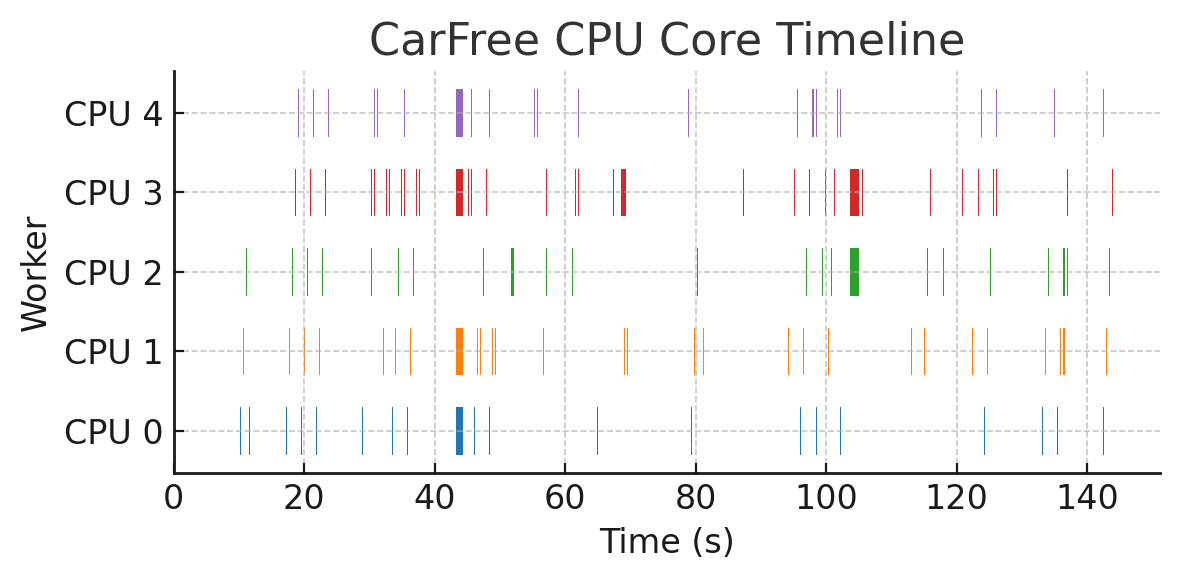
\includegraphics[width=\linewidth]{CarfreeCPUCoreTimeline.png}
    \caption{CarFree CPU Timeline}
    \label{fig:wide1}
  \end{subfigure}\hfill
  \begin{subfigure}{0.24\textwidth}
    \centering
    \includegraphics[width=\linewidth]{KittyCARLACPUcoreTimeline.png}
    \caption{Kitti-CARLA CPU Timeline}
    \label{fig:wide2}
  \end{subfigure}\hfill
  \begin{subfigure}{0.24\textwidth}
    \centering
    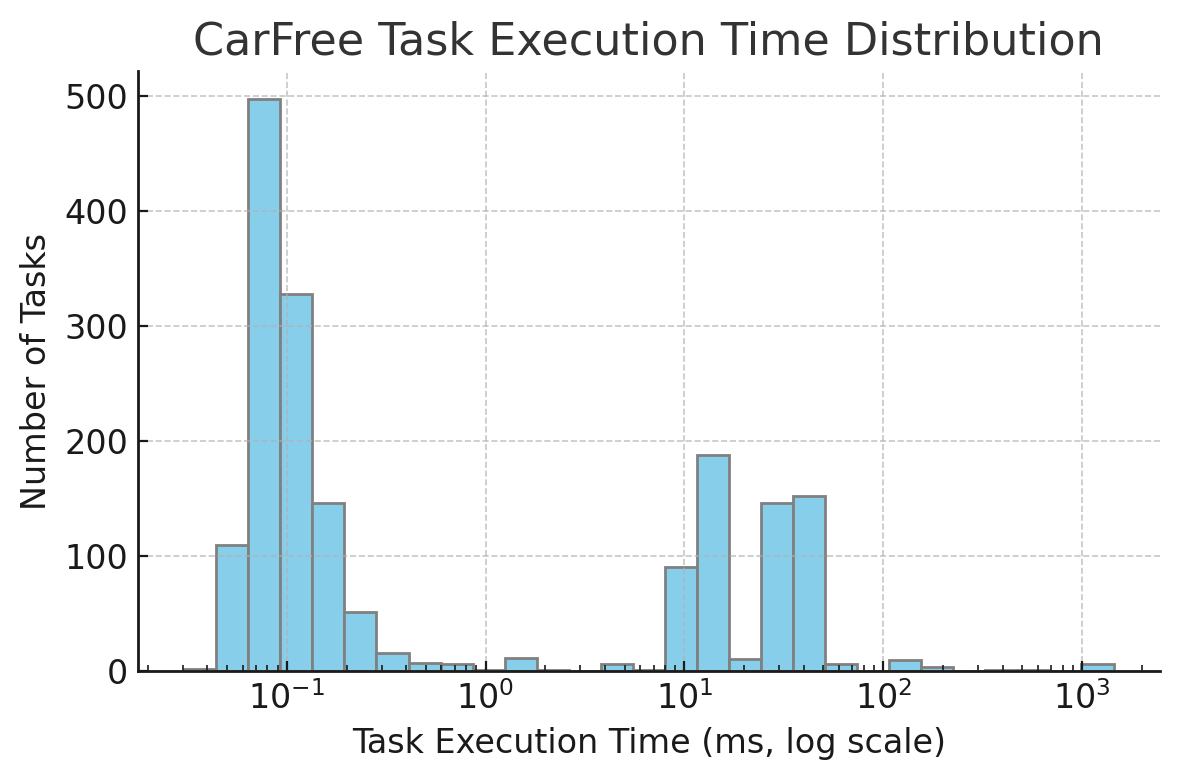
\includegraphics[width=\linewidth]{CarfreeExecutionTimeTimeline.png}
    \caption{CarFree Task Time}
    \label{fig:wide3}
  \end{subfigure}\hfill
  \begin{subfigure}{0.24\textwidth}
    \centering
    \includegraphics[width=\linewidth]{KittiCARLA distributiontimeline.png}
    \caption{Kitti-CARLA Task Time}
    \label{fig:wide4}
  \end{subfigure}

  \caption{CarFree vs Kitti-CARLA Analyses}
  \label{fig:four-wide}
\end{figure*}

\subsection{Cart-OnePiece as a Workload Characterization Tool}

For the purpose to show the use of this feature, it will be analyzed the Carfree and Kitti-CARLA enhanced scripts running on the I5 machine. The scheduling used again is the LWS that evenly distributes the workload between cores. Scheduling analyses will be done in the next section. Carfree generates tasks for 2d object detection and annotation. This creates around 1800 tasks, short in its majority for file writing and a few longer detection tasks. On the other hand, Kitti-CARLA emphasizes LiDAR point-cloud processing and georeferencing. In the simulation this workload issues 100 heavy tasks in a short burst saturating all the CPUs. Figure \ref{fig:four-wide} shows the results.


In the CarFree and Kitti-CARLA CPU core timelines, each row represents a CPU core that is called a worker in the StarPU. The colored bars show the execution intervals of the tasks in each core. The CarFree timeline in Figure \ref{fig:wide1} is sparse, tasks are intermittent, and rarely engage all cores simultaneously. At most 4 out of 5 cores execute tasks concurrently, reflecting low concurrency and utilization. In contrast, the Kitti-CARLA timeline in Figure \ref{fig:wide2} is almost completely occupied. Tasks are launched almost simultaneously in all cores.

The distribution of CarFree tasks in Figure \ref{fig:wide3} shows a bimodal nature reflecting two types of tasks: a large peak at around
$10^{-1}\,\text{ms}$ corresponds to hundreds of ultra-short file-write tasks, while a smaller cluster around $10^{1}$–$10^{3}\,\text{ms}$ represents the longer detection tasks. This heavy-tailed execution-time distribution is typical for pipelines with many trivial tasks plus a few expensive ones.  Consequently, the mean execution time (13.8 ms) is much higher than the median (0.13 ms), driven by these rare long-running tasks. On the other hand, in the Kitti-CARLA task execution time in Figure \ref{fig:wide4}, all tasks have high and similar runtimes, clustered between 1.0 and 1.8 s. Unlike CarFree, Kitti-CARLA shows a single-mode distribution with no short-task mode. This uniformity arises because every LiDAR processing task is computationally heavy and of similar complexity. 

\begin{table}[ht]
  \centering
  \caption{Scheduling Performance Metrics for CarFree}
  \label{tab:carfree_sched_perf}
  \renewcommand{\arraystretch}{1.5}
  \setlength{\tabcolsep}{3pt}
  \resizebox{\columnwidth}{!}{%
    \begin{tabular}{@{}l *{6}{P{1.5cm}}@{}}
      \toprule
      \rowcolor{myblue}
      \textbf{Scheduler}
        & \textbf{Tasks}
        & \textbf{Makespan (s)}
        & \textbf{Throughput (tasks/s)}
        & \textbf{Mean Task Dur (ms)}
        & \textbf{Mean Queue Delay (ms)}
        & \textbf{Avg CPU Util (\%)} \\
      \midrule
        EAGER      & 1802 & 139.4 & 12.92 & 10.04 & 0.060 & 2.60 \\
        DM         & 1809 & 141.1 & 12.82 & 12.28 & 0.244 & 3.15 \\
        HETEROPRIO & 1798 & 141.1 & 12.74 & 11.44 & 0.130 & 2.91 \\
        PRIO       & 1801 & 141.3 & 12.74 & 11.12 & 0.062 & 2.83 \\
        LWS        & 1802 & 141.7 & 12.71 & 13.62 & 0.399 & 3.46 \\
        WS         & 1801 & 142.3 & 12.66 & 11.16 & 0.361 & 2.82 \\
        DMDA       & 1816 & 143.6 & 12.65 & 13.49 & 0.215 & 3.41 \\
        RANDOM     & 1810 & 145.3 & 12.46 & 15.17 & 3.307 & 3.78 \\
      \bottomrule
    \end{tabular}%
  }
\end{table}




\subsection{Cart-OnePiece as a Task Scheduling Tool}

For the purpose of the application of this feature of the Cart-OnePiece tool, the CarFree script and the I5 machine will be used, and the scheduling strategies will be changed. Although StarPU enables for the creation for the user own scheduling strategy, for the purpose to demonstrate the usefulness of the tool, it will be used the pre-defined StarPU scheduling strategies.

After running CarFree for 3000 frames for each scheduling strategy, the data compiled in Table \ref{tab:carfree_sched_perf} was generated. The total tasks executed, makespan, throughput, mean task execution duration, mean scheduling queue delay, and average CPU utilization were reported. These metrics capture both throughput efficiency and latency characteristics important for real-time ADV workloads \cite{Balasekaran2021}. All policies achieve similar total work (within 1\% tasks) and overall throughput (around 12.5 to 12.9 tasks per second), but differ in how evenly they use resources and how long tasks wait to be scheduled.


\begin{figure}[h]
\centering
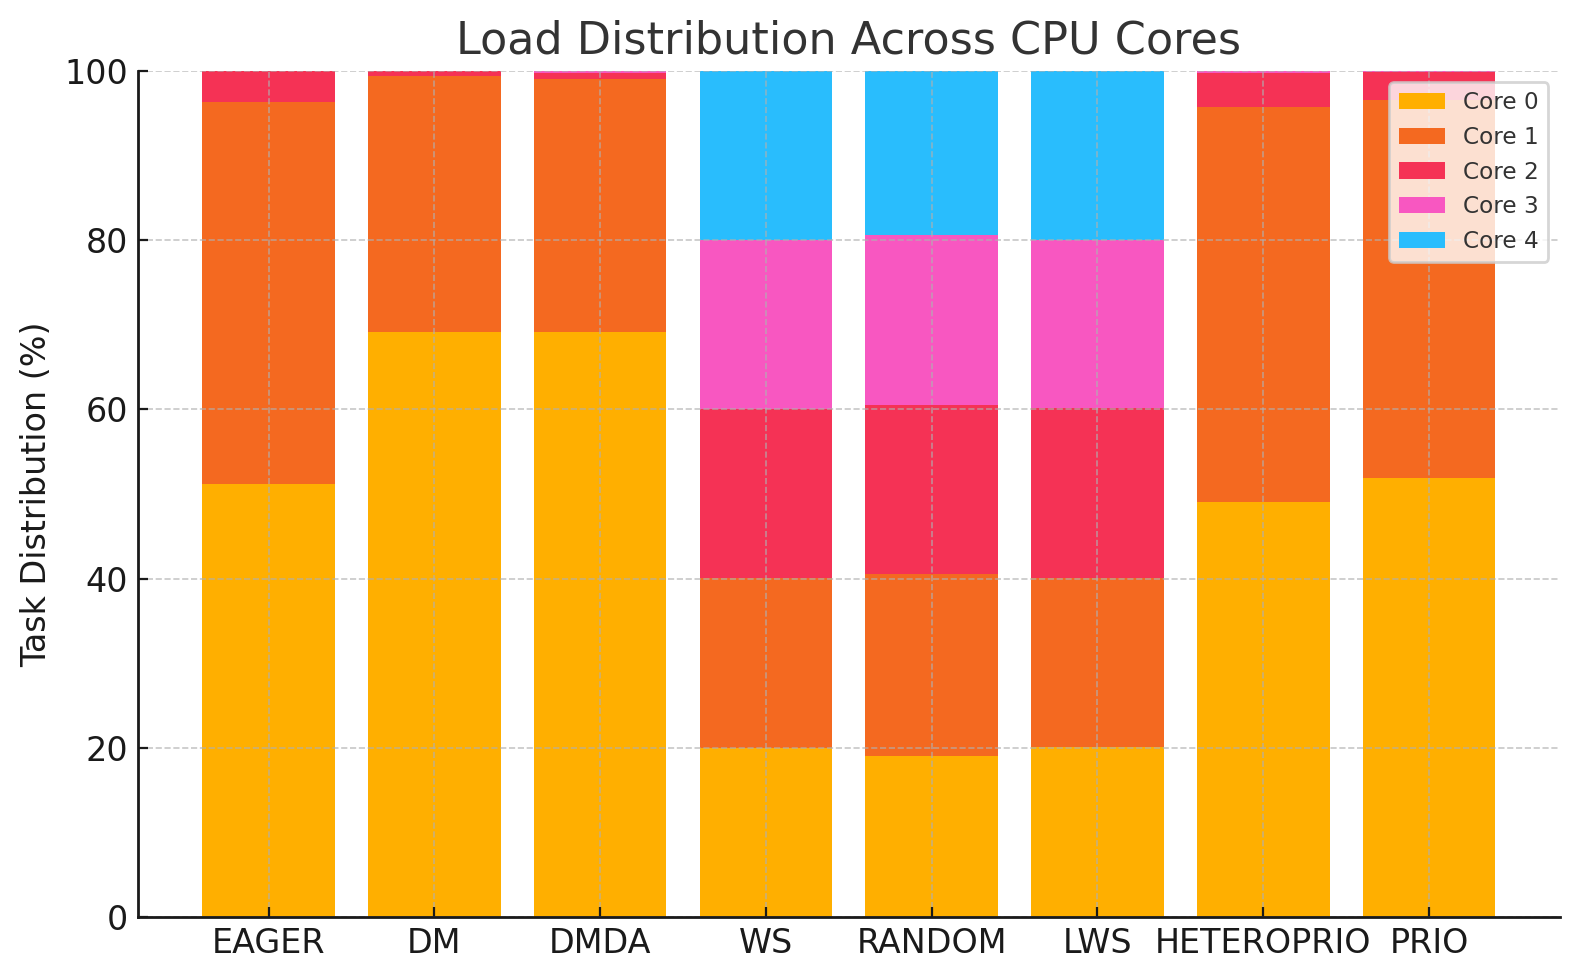
\includegraphics[width=\columnwidth, height=0.18\textheight]{CPU Utilization.png}
\caption{Load Distribution}
\label{fig:CPUtil}
\end{figure}


The Eager policy works faster, being the only one to finished its jobs below 141 seconds margin and achieves the highest throughput, while the Random policy is the slowest. The other strategies show similar results between 141 and 143 s, with very similar throughput. Another metric generated by the Cart-OnePiece tool is the load balance across the cores, which is illustrated in Figure \ref{fig:CPUtil}. Despite similar overall throughput, the policies differ in how they distribute work across the 5 CPU cores. While WS, LWS and RANDOM distribute the workload evenly between cores, DM and DMDA concentrate the workload in less cores. 

Seeing that RANDOM achieves the worst performance, it indicates that fairness alone is not sufficient for efficiency if scheduling decisions lack awareness of task readiness and data locality. In addition, seeing the distribution of workload in the more agreessive scheduler like PRIO and EAGER suggests that the scheduler has usually 1 to 2 tasks ready concurrently and that dispatch the work for the threads of the two first processors of the system.

\begin{figure*}[htbp]
  \centering
  % Row 1
  \begin{subfigure}{0.19\textwidth}
    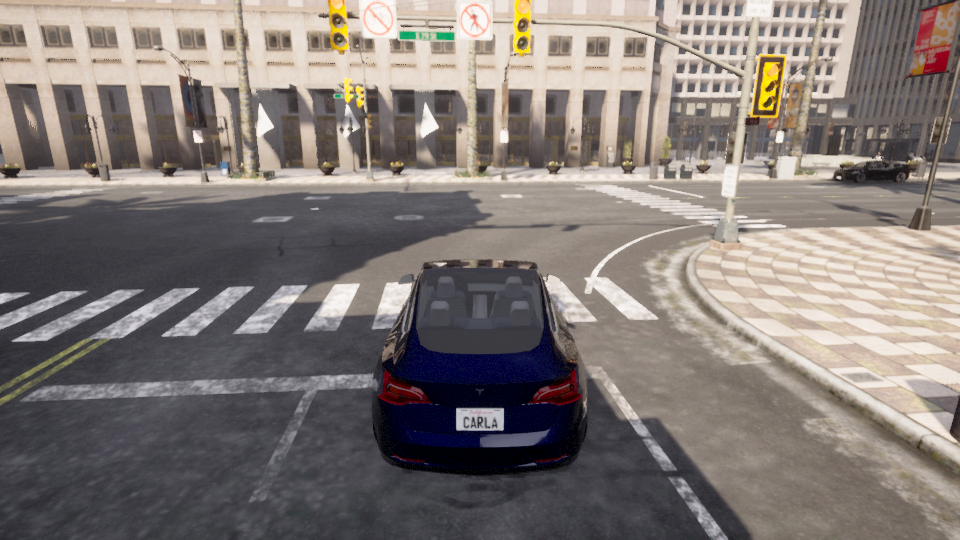
\includegraphics[width=\linewidth]{img1.png}
    \caption{Front RGB}
  \end{subfigure}\hfill
  \begin{subfigure}{0.19\textwidth}
    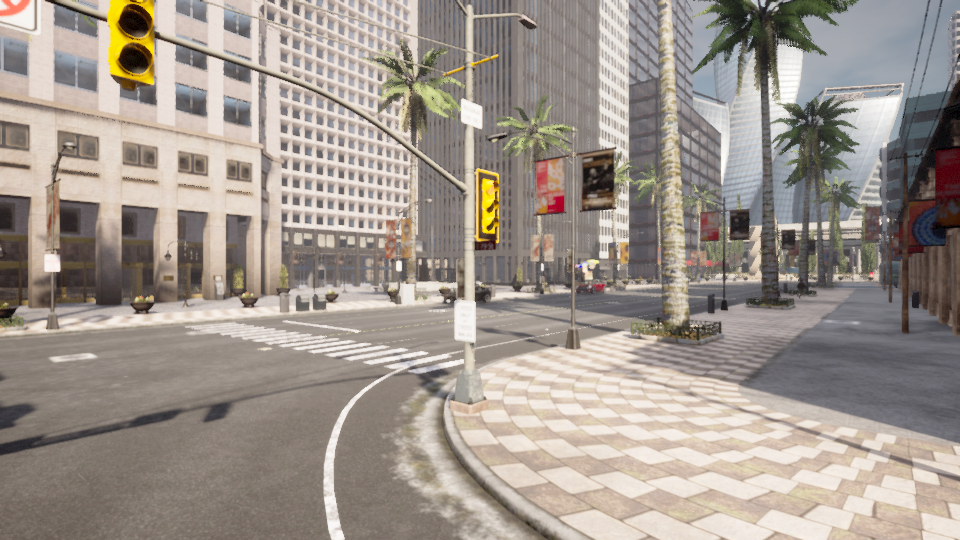
\includegraphics[width=\linewidth]{img2.png}
    \caption{Front Right RGB}
  \end{subfigure}\hfill
  \begin{subfigure}{0.19\textwidth}
    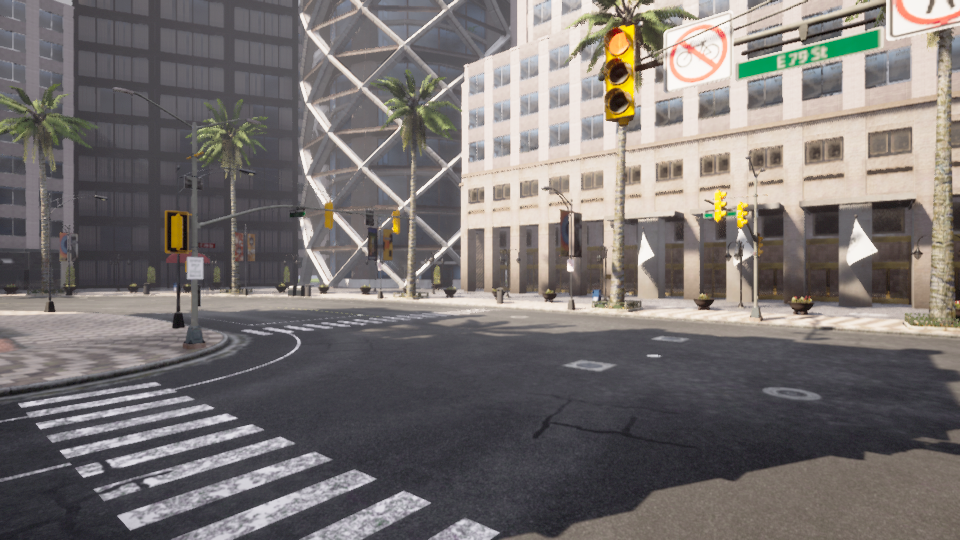
\includegraphics[width=\linewidth]{img3.png}
    \caption{Front Left RGB}
  \end{subfigure}\hfill
  \begin{subfigure}{0.19\textwidth}
    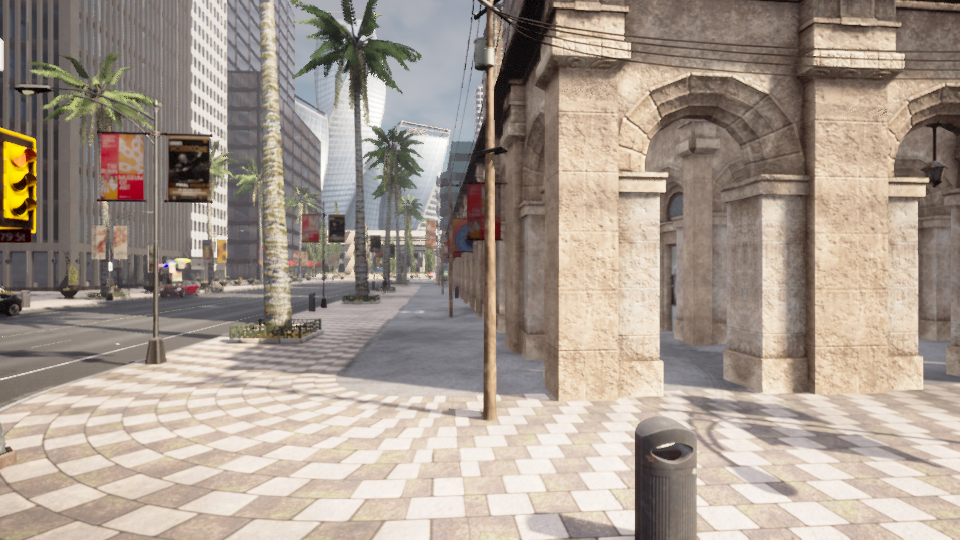
\includegraphics[width=\linewidth]{img4.png}
    \caption{Right RGB}
  \end{subfigure}\hfill
  \begin{subfigure}{0.19\textwidth}
    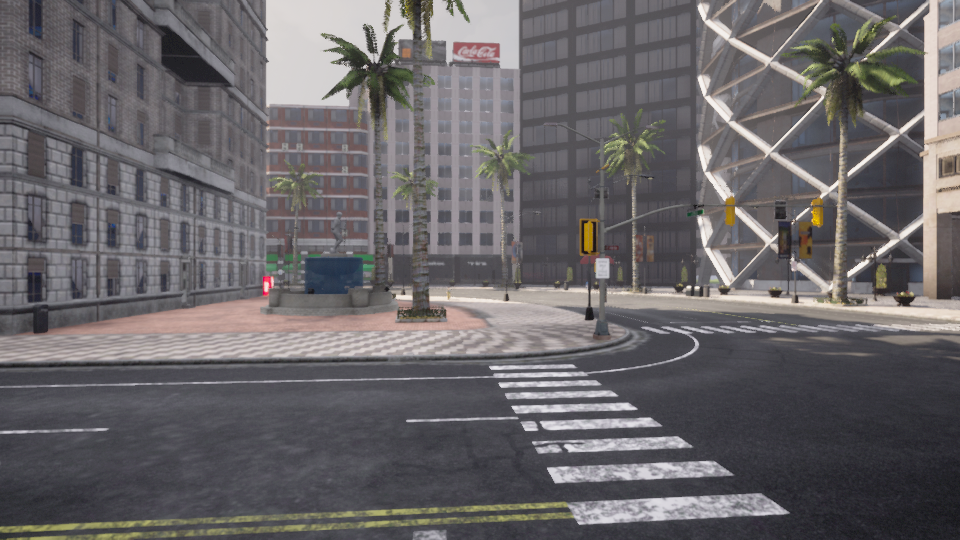
\includegraphics[width=\linewidth]{img5.png}
    \caption{Left RGB}
  \end{subfigure}

  \vspace{1em} % spacing between rows

  % Row 2
  \begin{subfigure}{0.19\textwidth}
    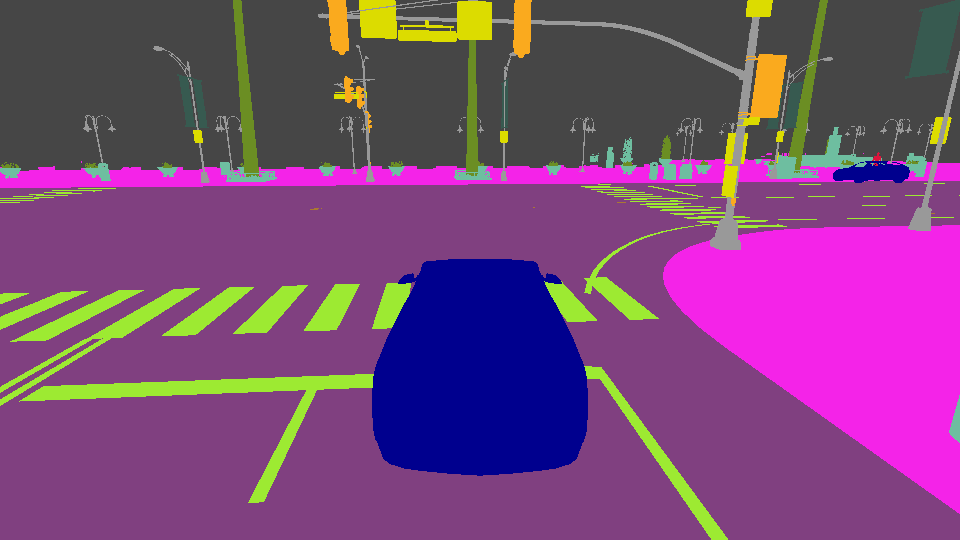
\includegraphics[width=\linewidth]{img6.png}
    \caption{Front SS}
  \end{subfigure}\hfill
  \begin{subfigure}{0.19\textwidth}
    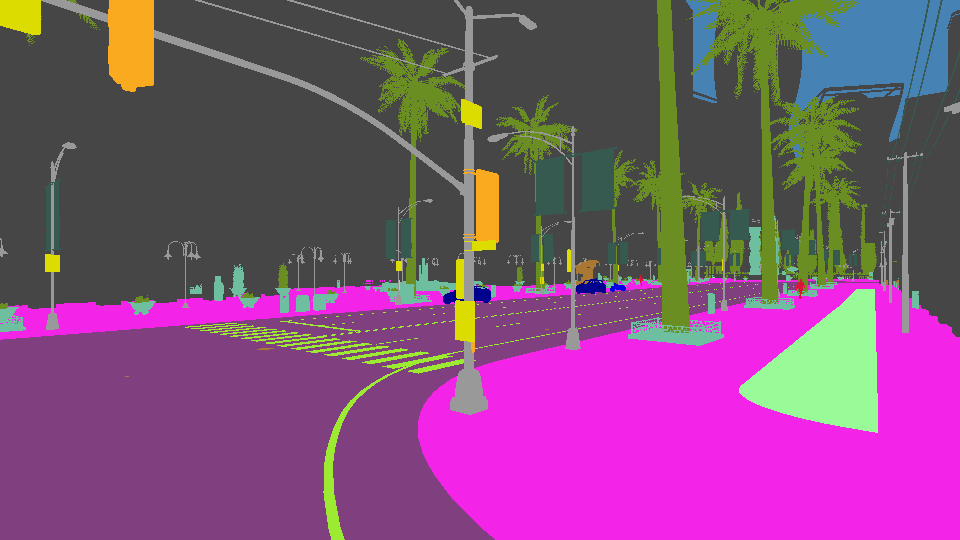
\includegraphics[width=\linewidth]{img7.png}
    \caption{Front Right SS}
  \end{subfigure}\hfill
  \begin{subfigure}{0.19\textwidth}
    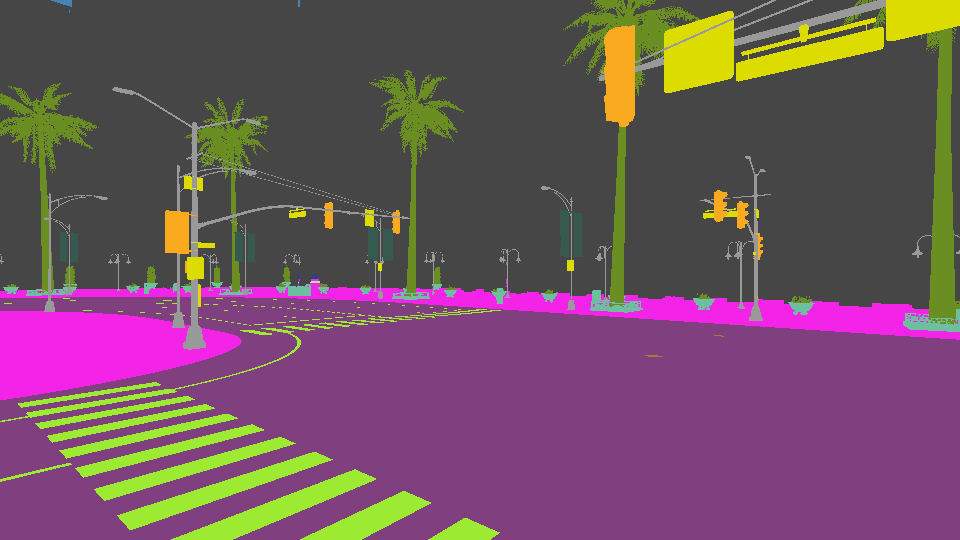
\includegraphics[width=\linewidth]{img8.png}
    \caption{Front Left SS}
  \end{subfigure}\hfill
  \begin{subfigure}{0.19\textwidth}
    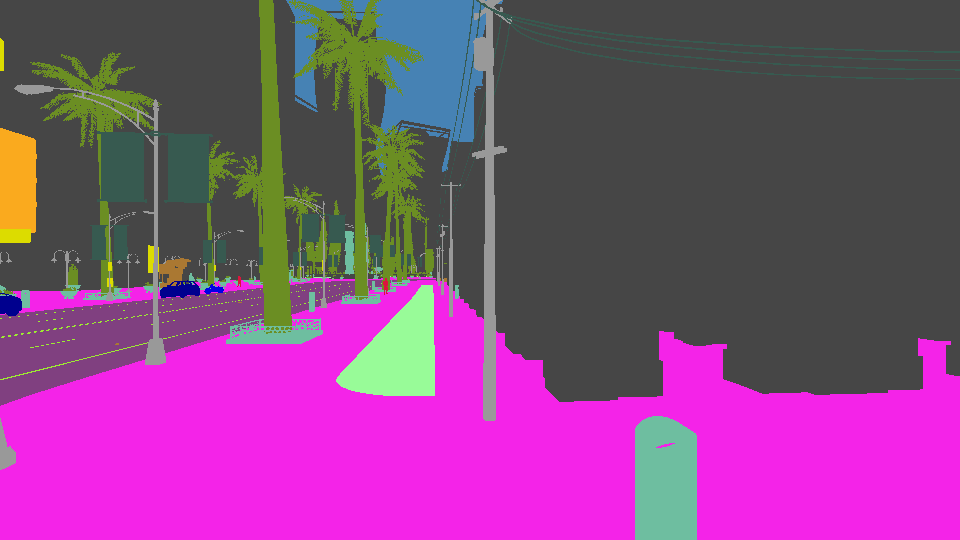
\includegraphics[width=\linewidth]{img9.png}
    \caption{Right SS}
  \end{subfigure}\hfill
  \begin{subfigure}{0.19\textwidth}
    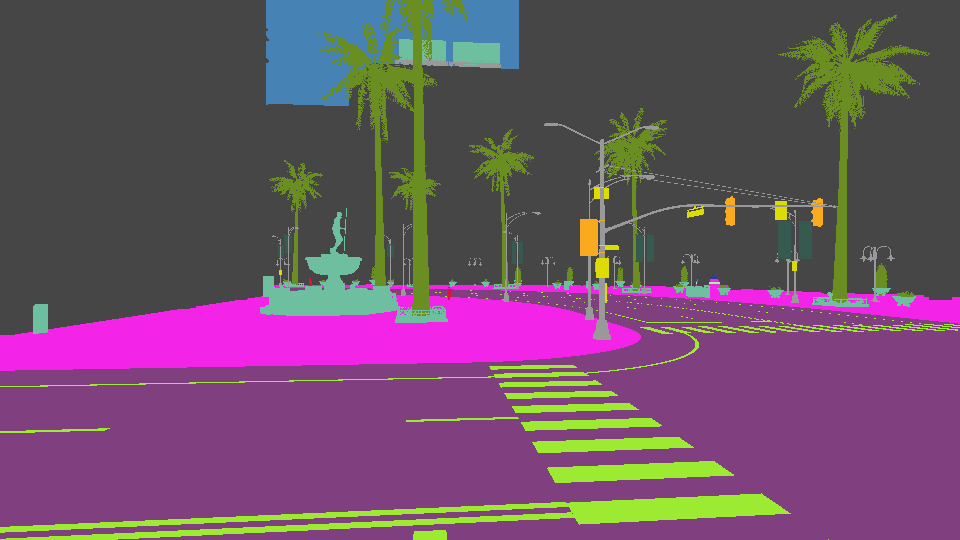
\includegraphics[width=\linewidth]{img10.png}
    \caption{Left SS}
  \end{subfigure}

  \caption{Data Collected From Cameras in Carfree}
  \label{fig:ten-subfigures}
\end{figure*}


\subsection{Cart-OnePiece as a Dataset Enhancer}

As described in the previous sections, Cart-OnePiece increases data collection to get close to what happens in the real world. Figure \ref{fig:ten-subfigures} illustrates samples from the enhanced Carfree dataset, showcasing high-fidelity synthetic images paired with their semantic segmentation (SS) annotations, reflecting realistic and detailed urban driving scenarios. The original Carfree script uses two cameras and this enhanced version applies 10 cameras in total, being 5 rgb and 5 semantic segmentation.

This reflects the Waymo Perception Dataset \cite{sun2020} that mimics its cameras positions. To reflect real world situations it was spawned together in the begging of the simulation 50 pedestrians and 30 vehicles in the TOWN10HD that is the name of this CARLA simulator town scenario. The tasks of collecting annotation to generate bounding box were collected successfully, getting annotation for pedestrians and vehicles for all new generated images.

\subsection{Limitations}

The version used of the CARLA simulator officially supports only Ubuntu 20.04 and Python version 3.8 {\cite{carla2025manual}}, although the API for Python version 3.10 could be found\cite{carla2025pypi}. As the latest release of this Ubuntu version was in 2020 and its long-term support ended in May 2025 it became incompatible with many up-to-date libraries, especially some use by the StarPU framework for profiling.  CARLA simulator has released a new version running in Unreal Engine 5 that supports Ubuntu 22.04 but the I5 machine setup could barely open the simulations, and the specifications require at least a machine with a 16gb dedicated GPU only to run the application. 

In addition, the I5 machine has just enough processing power to run the enhanced version of the scripts, needing to keep at minimum the use of the machine to any other processes while running the simulations. In addition, StarPU python binding presented a limitation on the API to profiling the application compared to C and C++. Furthermore, StarPU could use any Python version, but above 3.12 version it loses the use of a function that returns a future object necessary to many functionalities of the API.


\section{Related Work}
This section summarizes existing research on synthetic dataset generation, workload characterization, and task scheduling specifically for ADV, highlighting key approaches and limitations addressed by the proposed Cart-OnePiece tool.
\subsection{Synthetic Dataset Generation with CARLA}
CARLA has emerged as a popular platform for creating synthetic datasets due to its open-source nature, realistic rendering capabilities, and support for various sensors. The Kitti-CARLA dataset \cite{Deschaud2021Kitti-CARLA:Simulator}, for instance, replicates the sensor configuration of the real-world Kitti dataset within the CARLA environment. This enables researchers to train and evaluate algorithms on synthetic data while maintaining consistency with a well-established benchmark (Deschaud, 2021). The authors implemented pipelines based on deep learning architectures, such as YOLO for object detection and UNet for segmentation. CarFree \cite{Jang2022Carfree:Simulator} uses CARLA's automatic scene labeling to efficiently generate datasets for object detection. This dataset uses RetinaNet and Faster R-CNN as baseline detection models.

CARLA-GeAR \cite{Nesti2024CARLA-GeAR:Models} is designed to evaluate the adversarial robustness of perception models, generating image pairs with and without adversarial perturbations. ResNet-50 and YOLOv3 are used to evaluate performance degradation under adversarial attacks. ParisCARLA3D \cite{deschaud2021} combines real-world LiDAR data with synthetic data from CARLA to facilitate 3D mapping and object detection research. The dataset supports tasks including SLAM and 3D object detection using point-based neural architectures like PointNet++. CARLA-Loc \cite{Han2023CARLA-Loc:Environments} focuses on generating synthetic datasets for SLAM, featuring full-stack sensor setups and challenging environmental conditions.

Our approach differs from the sense of trying to bring reality to the dataset generation by copying the configuration of a working prototype and improving existing datasets to reflect more realistic generated data.

\subsection{Autonomous Vehicles Workload Characterization }

Several studies have focused on characterizing the workload of specific ADV components, such as perception, planning, and control \cite{Tang2022CharacterizationEdge, Liu2023COLA:Systems}. These characterizations often involve analyzing CPU utilization, memory footprint, memory bandwidth, and I/O requirements of these components under various driving conditions. Other works focus on end-to-end system characterization, considering the interplay between different ADV modules and their impact on overall performance \cite{Gog2021Pylot:Vehicles,Maity2021Chauffeur:Systems}.

Existing ADV benchmarks, such as CAVBench \cite{wang2018}, provide a suite of workloads and metrics to evaluate the performance of connected and autonomous vehicle systems. These benchmarks often include a variety of real-time and offline applications, reflecting the diverse computing requirements of ADVs. Edge AIBench 2.0 \cite{Hao2022EdgeSystems} is a scalable autonomous vehicle benchmark for IoT–Edge–Cloud systems. However, existing benchmarks often lack a scenario-level view, concentrating on specific algorithms or hardware performance.

Many works were also found to develop new scheduling strategies for ADV \cite{Xu2022AoI-centricSystems, Balasekaran2021, Yao2021, Yang2023BriefPruning} and one to explore scheduling strategies in ADV \cite{Silva2025TaskRuntime} but to the best of our knowledge the Cart-OnePiece tool proposed is the first work that would connect dataset generation and ADV workload and task scheduling analyzes in one tool only.


\section{Conclusion and Future Work}\label{SCM}
This paper introduced Cart-OnePiece, a novel integrated tool that enhances synthetic datasets, characterizes workload, and benchmarks task scheduling specifically made for ADV but that could be used to any other application. Through detailed analyses using the CARLA simulator and StarPU runtime, the relevance of this tool was demonstrated to analyze machine performance, task scheduling, and characterize the workload for ADV perception systems.

 Future research will focus on expanding workload characterization to include a wider range of tasks and metrics, the use of hardware accelerator data to improve the system analyses, and to explore new version of the software applied in this work.  In addition, the development of a procedure for the creation of a user-defined task scheduling policy for the Cart-OnePiece user could be a very important addition to it.

By addressing these areas, future research can further enhance the effectiveness and robustness of autonomous vehicle perception systems.

\begin{comment}
\subsection{Authors and Affiliations}

A minimum of one author is required for all conference articles. Author names 
should be listed starting from left to right and then moving down to the 
next line. This is the author sequence that will be used in future citations 
and by indexing services. Names should not be listed in columns nor group by 
affiliation. Please keep your affiliations as succinct as possible (for 
example, do not differentiate among departments of the same organization).


\subsection{Identify the Headings}

Headings, or heads, are organizational devices that guide the reader through 
your paper. There are two types: component heads and text heads.

Component heads identify the different components of your paper and are not 
topically subordinate to each other. Examples include Acknowledgments and 
References and, for these, the correct style to use is ``Heading 5''. Use 
``figure caption'' for your Figure captions, and ``table head'' for your 
table title. Run-in heads, such as ``Abstract'', will require you to apply a 
style (in this case, italic) in addition to the style provided by the drop 
down menu to differentiate the head from the text.

Text heads organize the topics on a relational, hierarchical basis. For 
example, the paper title is the primary text head because all subsequent 
material relates and elaborates on this one topic. If there are two or more 
sub-topics, the next level head (uppercase Roman numerals) should be used 
and, conversely, if there are not at least two sub-topics, then no subheads 
should be introduced.


\subsection{Figures and Tables}

\paragraph{Positioning Figures and Tables} Place figures and tables at the top and 
bottom of columns. Avoid placing them in the middle of columns. Large 
figures and tables may span across both columns. Figure captions should be 
below the figures; table heads should appear above the tables. Insert 
figures and tables after they are cited in the text. Use the abbreviation 
``Fig.~\ref{fig}'', even at the beginning of a sentence.

\begin{table}[htbp]
\caption{Table Type Styles}
\begin{center}
\begin{tabular}{|c|c|c|c|}
\hline
\textbf{Table}&\multicolumn{3}{|c|}{\textbf{Table Column Head}} \\
\cline{2-4} 
\textbf{Head} & \textbf{\textit{Table column subhead}}& \textbf{\textit{Subhead}}& \textbf{\textit{Subhead}} \\
\hline
copy& More table copy$^{\mathrm{a}}$& &  \\
\hline
\multicolumn{4}{l}{$^{\mathrm{a}}$Sample of a Table footnote.}
\end{tabular}
\label{tab1}
\end{center}
\end{table}

\begin{figure}[htbp]
\centerline{
\includegraphics{figs/fig1.png}}
\caption{Example of a figure caption.}
\label{fig}
\end{figure}

Figure Labels: Use 8 point Times New Roman for Figure labels. Use words 
rather than symbols or abbreviations when writing Figure axis labels to 
avoid confusing the reader. As an example, write the quantity 
``Magnetization'', or ``Magnetization, M'', not just ``M''. If including 
units in the label, present them within parentheses. Do not label axes only 
with units. In the example, write ``Magnetization (A/m)'' or ``Magnetization 
\{A[m(1)]\}'', not just ``A/m''. Do not label axes with a ratio of 
quantities and units. For example, write ``Temperature (K)'', not 
``Temperature/K''.



\section{Reference Formatting}

Please number citations consecutively within 
brackets~\cite{IEEEexample:conf_typical, IEEEexample:TBParticle}. The 
sentence punctuation follows the bracket~\cite{IEEEexample:article_typical}. 
Refer simply to the reference 
number, as in \cite{IEEEexample:bookwitheditor}---do not use 
``Ref. \cite{IEEEexample:bookwitheditor}'' or
``reference \cite{IEEEexample:bookwitheditor}'' except at 
the beginning of a sentence: 
``Reference \cite{IEEEexample:bookwitheditor} was the first $\ldots$''

Number footnotes separately in superscripts. Place the actual footnote at 
the bottom of the column in which it was cited. Do not put footnotes in the 
abstract or reference list. Use letters for table footnotes.


\paragraph{Sorting \& Format Definition}

The included \texttt{IEEEtranS.bst} format is \textbf{required}, as this 
sorts papers alphabetically by surname of the first author. 
Do \emph{not} use a different sorting.


\paragraph{Author Names}

List all author names explicitly --- do not use 
``et al.''. Papers that have not been published, even if they have been 
submitted for publication, should be cited as ``unpublished''. Papers 
that have been accepted for publication should be cited as ``in press''. 
Capitalize only the first word in a paper title, except for proper nouns and 
element symbols.

For papers published in translation journals, please give the English 
citation first, followed by the original foreign-language citation.



\section*{Acknowledgments}

The preferred spelling of the word ``acknowledgments'' in America is without 
an ``e'' after the ``g''. Avoid the stilted expression ``one of us (R. B. 
G.) thanks $\ldots$''. Instead, try ``R. B. G. thanks$\ldots$''. Put sponsor 
acknowledgments in the unnumbered footnote on the first page.
\end{comment}

\bibliographystyle{IEEEtranS}
\bibliography{reference}


\end{document}